\documentclass{iopjournal}
\usepackage{amsmath,amssymb}
% figures share their page with text: no float page unless it is mostly full, at most one float on top
\renewcommand{\topfraction}{0.7}
\renewcommand{\bottomfraction}{0.5}
\renewcommand{\textfraction}{0.3}
\renewcommand{\floatpagefraction}{0.8}
\setcounter{topnumber}{2}
\setcounter{totalnumber}{3}
\usepackage{longtable,booktabs,array,calc}
\usepackage{textcomp}
\providecommand{\tightlist}{\setlength{\itemsep}{0pt}\setlength{\parskip}{0pt}}
\def\LTcaptype{table}

\begin{document}

\articletype{Paper}

\title{Accountable experiments: autonomous measurement with error bounds set in advance}

\author{Petrus H. Zwart$^{1,*}$}
% TODO: co-authors, ORCID iDs (\orcid{...})

\affil{$^1$Molecular Biophysics and Integrated Bioimaging Division, Lawrence Berkeley National Laboratory, Berkeley, CA, USA}

\affil{$^*$Author to whom any correspondence should be addressed.}

\email{phzwart@lbl.gov}

\keywords{accountable experiments, autonomous experimentation, distribution-free risk control, conformal prediction, adaptive sampling, hierarchical design, self-driving laboratories}

\begin{abstract}
%did not touch the abstract - will only do this when we are fully done
An autonomous experiment decides where to measure and where not to, and a skipped site seldom can be revisited once sample, beam time or reagent is spent. Each skip therefore needs a bound on how often skips are wrong, fixed in advance. The model steering the campaign cannot supply that bound. It selects the sites on which its own error is then judged, a circular analysis, and a coherent Bayesian forecaster assigns probability one to its own calibration, so its stated error rate confirms itself. We show one way to break this cycle. A specification fixed before the campaign names a plan of sites, the claims under which a site may be skipped, and a budget on skip errors held with a stated confidence. In each round a model is fitted and frozen, a uniform calibration sample is measured, and conformal thresholds set from its labels decide the skips. The bound is probably approximately correct (PAC): the share of a round skipped in error stays within the budget in at least the stated fraction of campaigns, whatever the model. On a fully measured NaCl microdiffraction scan, with one frozen Gaussian process and calibration sample shared by both cuts, conformal thresholds kept the stated rate in 78 \% to 89 \% of 80 campaigns, against a target of 80 \%, with each of three kernels and with a predictor guessing at random. Cut by its own uncertainty, the process kept its rate in 69 \% to 100 \% with a noise term and in none with a kernel that assumed a smooth map; with that kernel the thresholds measured 723 sites against 317, and the map refitted from them was better in each of 20 designs. Levels kept their budget at the stated confidence on an infrared map and a synthetic scattering map as well. A held-out audit gives the finished map its own bound.
\end{abstract}

\hypertarget{sec:1}{%
\section{Introduction}\label{sec:1}}

Autonomous experiments now decide where to measure and where not to. At synchrotron beamlines, Gaussian-process surrogates choose the next sample position or composition, and measurement, analysis and decision run as one closed loop \cite{Noack2019,Noack2020,Yager2023}. Self-driving laboratories search formulation and composition spaces in the same way \cite{Burger2020,Nazeri2026,Szymanski2023}. In the biosciences, probabilistic models recommend which bacterial strains to build next \cite{Radivojevic2020}, and laboratory automation keeps lowering the cost of handing experimental choices to machines \cite{Tom2024}. Each decision to measure is also a decision to leave something unmeasured. In a recent closed-loop scattering study, for example, the phases of a ternary polymer blend were mapped by choosing 65 of 5151 grid compositions, so that 98.7 \% of the map is a prediction \cite{Upreti2026}.

Handing the choice of where to measure, and where not, to a model requires each of these actions and inactions to be justified at decision time. A measurement uses resources and an opportunity that may not return; a skipped site usually stays unknown, since sample degradation, an ended beam time or a spent reagent prevents a later visit. The reason for each skip, and the risk it carries, therefore needs to be documented when the skip is decided. Fields that hand consequential decisions to automated systems already ask for this: guidance on AI risk asks for traceable decisions and documented responsibility \cite{NIST2023}, regulation of high-risk systems requires automatic records of their operation \cite[Art. 12]{EU2024}, and audit frameworks ask for evidence that can be checked against stated expectations \cite{Raji2020}. Accountability, in this sense, means that a decision can be checked against expectations stated before it was taken. Here we argue for the same practice in autonomous experiments: before a decision is taken, a bound is attached to it, so that every skip carries an error bound stated before it was made. An account given after the campaign, such as the measurement of a random subset of new locations across the finished map, validates decisions already spent and reports a final error; it is useful, and it cannot change a decision that has been taken. For a mapping campaign the consequential decisions are where not to measure, and accountability asks that they be made so as to reflect a policy or goal fixed before the campaign.

The model that steers a campaign cannot supply that bound itself. It selects the sites it is fitted on and then judges its error on the same sites, a circular analysis that biases the estimate whatever the model \cite{Kriegeskorte2009}. Bayesian coherence tightens the loop: a coherent forecaster assigns prior probability one to its own long-run calibration \cite{Dawid1982}, so its stated error rate confirms itself, and cross-validation inherits the bias of the sites the model chose \cite{Barber2021,Fannjiang2022}. An error found afterwards is laid at the door of the kernel, the hyperparameters or the noise model, each a choice that could have been made otherwise, whether or not checking it was practical at run time. A guarantee that covers such choices has to be paid for in advance, before it is known whether the model is right.

Figure~\ref{fig:1} illustrates the problem on a fully measured NaCl microdiffraction scan, where a Gaussian-process regressor (GPR) decides which sites to visit. In each round of the simulation, a GPR is fitted on the sites measured so far and frozen, and the sites of the next round of the design become available; 40 of them, drawn at random, are measured and set aside for calibration. The remaining sites are ranked by the model's probability that a skip would be in error, because the presence of the (200) diffraction line is predicted wrongly or because its width cannot be interpolated within tolerance, and the least safe sites are measured. How far down this ranking sites may be skipped is governed by a policy fixed in advance: at most a fifth of each round skipped in error, held in at least 80 \% of campaigns. Three versions of the GPR are compared: one with length scale and noise fitted from the data, one with the noise term fixed at a value that is too low, and one with, in addition, the length scale held at a value that is too large. Run over 80 designs and checked against the full scan in hindsight, the cut set by the GPR's own probabilities met the policy only as often as its kernel allowed: with the noise fitted, in 88 \% to 100 \% of campaigns, more often than the 80 \% asked for, so that measurements were spent the policy did not require; with the noise too low, in as few as 69 \% of campaigns; and with the length scale too large, in none. The reason is well known: the predictive probabilities of a GPR are calibrated only when its kernel suits the data, and hyperparameters estimated from the data can leave them too cautious or overconfident \cite{Karvonen2020}. Thresholds set instead from an exact count of the errors the ranking makes among the 40 calibration sites kept the policy close to 80 \% with every kernel, and with a predictor guessing at random; the model decided only how many sites were measured (Section~\ref{sec:5-2}). With the overconfident kernel, the map refitted from the sites it chose was worse in each of 20 designs: about 30 \% of the scan was predicted outside tolerance, against 24 \% when the conformal thresholds set the cut.

\begin{figure}[tbp]
\centering
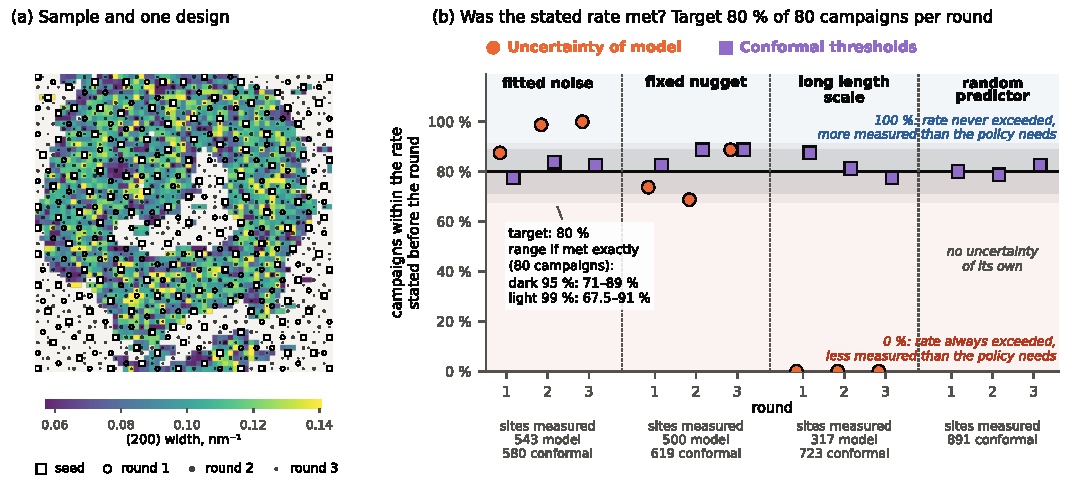
\includegraphics[width=\textwidth,height=0.44\textheight,keepaspectratio]{figures/fig_hook4}
\caption{Rates of skip errors stated before each round and realised, under the uncertainty of a model and under conformal thresholds. A fully measured NaCl microdiffraction scan, claim on the presence and width of the (200) line (tolerance 0.02 nm\ensuremath{^{-1}}), stated rate of at most a fifth of each round skipped in error, held with confidence 0.80. Each of 80 hierarchical designs, about 1075 sites, measures its coarsest levels as a seed, about 143 sites, and decides each of its three finer levels in one round. In every round the same Gaussian process, fitted on the sites measured so far and frozen, ranks the sites of the round, and a uniform calibration sample of 40 is measured; the cut on the remaining sites is set by the uncertainty of the model (circles, from its joint predictive distribution) or by conformal thresholds from the calibration labels (squares). Each cut is shown in the campaigns it drives. (a) Width of the (200) line over the scan, with the seed and three rounds of one design. (b) Share of campaigns whose realised skip errors stayed within the number stated before the round. The target is the confidence $c = 1 - \delta$ with which the budget \ensuremath{\varepsilon} is held. A cut that meets it sits near 80 \%; near 100 \% the stated rate is never exceeded, so more is measured than the policy needs, and near 0 \% it is always exceeded, so less is measured than the policy needs. Kernels: noise level fitted; noise fixed at 10\ensuremath{^{-}}\ensuremath{^{4}} of the variance; noise fixed and length scale held at 1 mm or more. Random predictor: each site copies a measured site chosen at random, sites are ranked at random, and nothing is stated about its errors. Grey bands: central 95 \% (dark) and 99 \% (light) range of the share for a method meeting the target exactly, binomial over 80 campaigns. Sites measured: mean over 80 campaigns, seed and calibration included.}\label{fig:1}
\end{figure}

Fixing bounds before the decision is established practice wherever a decision cannot wait for hindsight. In acceptance sampling, a lot is accepted or rejected from a sample drawn at random, with the sample size and the number of defects allowed in it fixed before inspection, so that the risk of accepting a bad lot is known at acceptance \cite{DodgeRomig1959}. Group sequential clinical trials fix in advance how the type I error is spent over interim analyses, so that a trial may stop early with its error rate intact \cite{LanDeMets1983}, and registered reports fix hypotheses and analyses before data are collected \cite{Chambers2013}. Design-based survey sampling places the randomness in a plan fixed in advance, so that statements about a finite population hold whatever its values \cite{Neyman1934,Cochran1977}. The mapping campaigns outlined here fit this pattern closely: the levels of the design are interim analyses, the failure probability can be spent across them, and each level is a lot accepted from a random sample.

This paper shows how a mapping campaign can be run so that every skip is covered by a bound fixed in advance. Optimisation campaigns, which search for an extremum instead of a map, raise different questions and are not treated here. Before the campaign starts, three things are written down. The first is the plan: the sites that would be measured if none could be skipped, which in spatial mapping are the sites at the finest spacing worth resolving. The second is the set of claims under which a site may be skipped, for example that its signal, or a quantity derived from it, can be interpolated within a declared tolerance, or that it holds nothing of interest. Every other site is measured. The third is a budget \ensuremath{\varepsilon} on the share of sites skipped under a false claim, together with the confidence $c$ with which that budget must hold. Because this work concerns ordered, continuous spaces that are expected to vary smoothly, the plan is a nested space-filling design \cite{Qian2009}. It is split into resolution levels, each filling the gaps of the coarser ones, and the coarsest levels are measured in full. The levels serve the formation of an image at every resolution; the guarantee only needs each level to be fixed before its calibration sample is drawn, and any other partition of the plan would serve it equally (Section~\ref{sec:3-1}).

Each finer level is decided in one round. A model is fitted to the sites measured so far, frozen, and used to rank the sites of the level by how safe a skip is. A sample of the level, drawn at random, is then measured, and conformal thresholds set from these measurements decide how far down the ranking sites may be skipped. The bound is therefore attached to the decision on a level before any of its sites is skipped, and it holds for any model, as long as the steps are taken in this order. In words, the share of a level skipped in error stays below \ensuremath{\varepsilon} in at least a fraction $c$ of campaigns: at \ensuremath{\varepsilon} = 0.20 and $c$ = 0.80, at most a fifth of a level is skipped in error, at least four times in five. Bounds of this kind are known as probably approximately correct (PAC) \cite{Valiant1984}. Because a campaign is run only once, this is the statement that matters to an experimenter; a bound on the average share holds over many campaigns, and single levels then exceed the budget far more often (Section~\ref{sec:5-1}). The statistics are standard finite-sample risk control \cite{Vovk2005,Bates2021,Angelopoulos2025}. What is new is how the experiment is posed: in a closed loop, every decision changes the data used to judge the next one, and fixing each level before its calibration sample is drawn lets the standard results apply. The model enters only through its ranking, so a poor model leads to more measurements, and, as Fig.~\ref{fig:1} shows, those measurements also give a better map. A held-out audit after the last level adds a bound on the finished map.

The approach is tested on three fully measured datasets, on which every skip can be checked: an infrared map of a bioreef sample, a NaCl microdiffraction scan \cite{ALSNaCl} and a synthetic small-angle scattering phase map. On all three, levels exceeded their budget no more often than the stated confidence allows. When the budget was required to hold on every level at once, it held in at least 90 \% of campaigns, at a cost of 13 \% to 41 \% more measurements. The choice of model and score set the number of measurements. The Gaussian process serves as an example: the guarantee rests on the calibration sample alone, and claims about the process concern this process on this scan. A live campaign is left for future work. Section~\ref{sec:2} places the work among adaptive mapping and distribution-free inference, Section~\ref{sec:3} describes the specification and its guarantee, Section~\ref{sec:4} the datasets and protocols, Section~\ref{sec:5} the results, and Section~\ref{sec:6} what the specification costs and what it covers.

\hypertarget{sec:2}{%
\section{Related work}\label{sec:2}}

\textbf{Adaptive mapping.} Scanning instruments spend most of their time on sites that add little to the final map, and adaptive acquisition puts that time where the map is uncertain or interesting. Gaussian-process regression drives autonomous small-angle scattering and diffraction mapping at synchrotron and neutron facilities \cite{Noack2019,Noack2020,Noack2021}, and steers robotic formulation of polymer blends through their scattering peak ratios \cite{Upreti2026}. Bayesian active learning maps phase diagrams of composition spreads on the fly at the beamline \cite{Kusne2020}. Dynamic sampling selects each new pixel of a point-wise image by the expected reduction in distortion and stops once an estimated distortion is reached \cite{Godaliyadda2018}. Scanning probe and electron microscopes run comparable loops of measurement, model update and choice of the next location \cite{Kalinin2021,Ziatdinov2022}. These methods judge the sites they leave out through the model that chose them.

\textbf{Distribution-free risk control.} Distribution-free inference attaches finite-sample statements to the output of an arbitrary predictor, with exchangeability of the calibration data as the only assumption \cite{Vovk2005,Angelopoulos2023}. Risk-controlling prediction sets bound the population rate of a chosen loss from a held-out sample with high probability over that sample, a PAC statement \cite{Bates2021,Park2020}, Learn-then-Test extends the bound to any family of decision rules searched in a fixed order or with a multiple-testing correction \cite{Angelopoulos2025}, and conformal risk control bounds an expected loss \cite{Angelopoulos2024}. Several risks can be controlled at once, and a path through a family of rules can be learned on part of the data \cite{LauferGoldshtein2023}. Conformal selection controls the false-discovery rate among the items a model selects \cite{Jin2023}, a statement close in spirit to a bound on skip errors among the skipped sites, and selective classification guarantees, with high probability, the risk of the predictions a model chooses to make \cite{Geifman2017}. The bound on a level is, at its core, the acceptance sampling of Section~\ref{sec:1}, which accepts a lot from a sample of fixed size with an allowed number of defects; risk-limiting audits apply the same logic to the count of an election \cite{LindemanStark2012}. The present work poses a skip as a claim about a site, so that the claims of a mapping campaign become the losses these methods control.

\textbf{Exchangeability in space.} Spatial data are dependent, and a calibration sample drawn from a map is exchangeable with the rest of the map only under conditions. Spatial conformal prediction obtains exact or approximate exchangeability from properties of the spatial process, for instance local approximate exchangeability around a prediction location for a broad class of processes \cite{Mao2024}. Design-based inference takes the opposite route and places the randomness in the sampling plan, so that statements about a finite population hold whatever the values in it \cite{Neyman1934,Cochran1977}; in model-assisted estimation a model improves precision while the design alone carries validity \cite{Sarndal1992}, and conformal prediction has been carried into this setting \cite{Vovk2013,Wieczorek2023}. Active inference uses a model to choose which items to label and keeps valid inference through known sampling probabilities \cite{ZrnicCandes2024}, a route that could let measured sites serve calibration as well. The campaign here follows the second route: a plan fixed level by level before each draw gives every level its population, and a uniform draw makes the calibration sample exchangeable with it, whatever the campaign did before, with no model of the spatial dependence.

\textbf{Adaptive sensing with guarantees.} Two recent lines of work bring calibrated uncertainty into the acquisition loop itself. Conformal intervals decide which pixels to re-scan in photon-limited scanning microscopy \cite{Ye2025} and when enough has been acquired in rate-adaptive sensing \cite{YangZhang2026}, both calibrated on data collected outside the running acquisition. Power-system security screening offers the closest construction outside imaging: a label-independent audit drawn from the current operating window guarantees the violation rate among contingencies that a cheap surrogate lets the operator skip, and the surrogate affects the cost of the guarantee and leaves its validity untouched \cite{Manoharan2026}. The present work guarantees each skip of a running scan by a claim, takes its calibration sample from the scan through the design, and checks every guarantee against fully measured truth.

\hypertarget{sec:3}{%
\section{Framework}\label{sec:3}}

\hypertarget{sec:3-1}{%
\subsection{Design and order of operations}\label{sec:3-1}}

An experiment declares before it starts the most it will measure and the finest detail it seeks. The plan, the design sites it would measure if none could be skipped, carries both: its finest spacing sets the resolution of the final map, and its sites bound the measurements. The same plan serves the guarantee. A finite-sample guarantee about skipped sites needs a calibration sample that is exchangeable with the sites it speaks for \cite{Vovk2005}. Here the design creates that exchangeability. The population of every level is fixed before its calibration draw, and a uniform random draw from that population is the only source of randomness the guarantee relies on, as in design-based survey inference \cite{Neyman1934,Cochran1977}. The guarantee needs no model of the spatial field or of the noise.

Here a hierarchical Poisson-disk design \cite{Bridson2007} lays out the plan in nested levels of increasing density. Any plan whose levels are fixed before their draws would serve the guarantee equally: a grid, independent uniform points, or a level drawn up from the sites already measured, such as the neighbourhood of sites found interesting. The hierarchy serves image formation: the sites up to any depth contain every coarser depth and form an evenly spread design at that resolution, so each map builds on the coarser maps and interpolation has well-placed support. Nesting and spread set the cost of a guarantee and play no part in its validity. Each completed level also yields a map at the spacing of its sites, in which every site is measured or predicted under a claim bounded on its level; a display map can be drawn afterwards with any interpolator. The coarsest levels form the seed and are measured in full. Each finer level is then processed once, in order, in five steps (Fig.~\ref{fig:2}):

\begin{enumerate}
\def\labelenumi{\arabic{enumi}.}
\tightlist
\item
  \emph{Fit.} The predictor and the scores are fitted on the sites measured so far.
\item
  \emph{Freeze.} Scores and predictor are fixed for every site of the level, and so is the decision rule: the family of thresholds, the budget and its split, and the number of calibration failures the level may allow.
\item
  \emph{Draw.} A calibration sample of \(m\) sites is drawn uniformly without replacement from the level, with randomness independent of everything else.
\item
  \emph{Calibrate.} The calibration sites are measured, their labels are evaluated against the frozen predictor, and the rule turns the labels into thresholds.
\item
  \emph{Decide.} Covered sites of the remainder are skipped and the others measured; every measured site joins the measured set for the next level.
\end{enumerate}

Step 5 is the action of the level: one decision, taken after the draw, on which of its sites are measured and which are skipped, and under which claim. The decision covers every site of the level at once, so the order in which the sites are then measured is free. The plan, together with the rule that decides each of its levels, is guaranteed to keep the budget of the specification on every level, at most a fraction \ensuremath{\varepsilon} of the sites skipped under a false claim, with probability at least c over its calibration draws; the failure probability 1 \ensuremath{-} c is divided among the levels when the plan is declared. Each action has its bound, and the record gives every site its reason.

\begin{figure}[tbp]
\centering
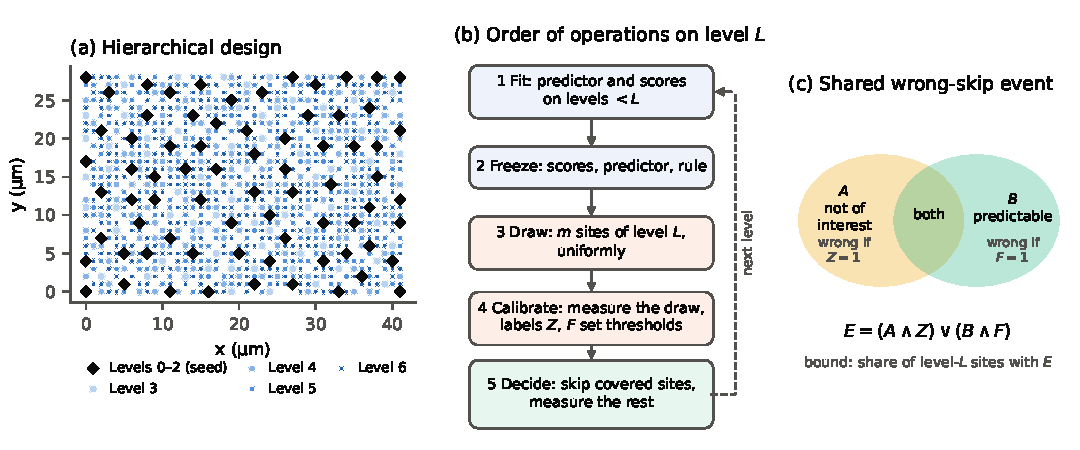
\includegraphics[width=\textwidth,height=0.44\textheight,keepaspectratio]{figures/fig1_schematic}
\caption{The workflow. (a) Hierarchical design of the IR map: levels 0--2 form the seed, and each finer level fills the gaps of the coarser ones. (b) The five steps on one level; the calibration draw is the only random element of the guarantee, and its labels are unseen until the rule is frozen. (c) The two claims: a skipped site is covered as not of interest (\(A\)), as predictable (\(B\)) or both, and the skip is wrong when a covering claim is false. The guarantee bounds the share of level-\(L\) sites at which the shared event \(E\) occurs.}\label{fig:2}
\end{figure}

Non-anticipation ties the steps together: nothing that shapes the guarantee on a level may depend on that level\textquotesingle s draw, except through the rule fixed in step 2. Three practices that look harmless break it, and Section~\ref{sec:5-1} shows each failing: refitting the scores on the calibration labels before the threshold is set, taking the calibration sample where the model is least sure, and keeping the most favourable of several draws. The condition concerns the draw and the rule. A score may use anything known before the draw, including physical models, other datasets or prior beliefs; a poor score costs measurements and leaves the guarantee intact.

Measuring one site must also leave the outcome of every other site unchanged. Radiation damage that spreads beyond the probed spot, or sample drift triggered by the measurement order, would let the draw alter the population it is meant to sample.

Given everything that precedes the draw of a level, its population, scores, labels and rule are fixed, so the guarantee holds conditionally on the history of the campaign and adaptivity across levels leaves it intact. Statements about several levels follow from the union bound; Appendix~\ref{app:A} states the conditions formally.

\hypertarget{sec:3-2}{%
\subsection{Claims and labels}\label{sec:3-2}}

A skip is useful only if it says something that a measurement could contradict. Two claims serve that purpose. The interest claim states that a site holds nothing of interest; its label \(Z(x) = 1\) marks a site whose measured spectrum meets the interest criterion of the dataset, such as a diffraction line standing clear of the noise. The interpolation claim states that a site is predictable; its label \(F(x) = 1\) marks a site where the prediction from the coarser levels misses the acceptance metric. The metric fixes what predictable means: agreement of the full spectrum within an envelope, or agreement of a quantity derived from it, such as a peak position or width, within a tolerance. Both labels are functions of the true spectrum, the one a single measurement returns, and of the frozen predictor. In a campaign they are known only at measured sites, and for this study they are known everywhere.

Each claim carries a score that orders the sites of a level from most to least safe to skip. The score has no other role: any function of the data available before the draw may serve, and its quality decides the number of measurements spent. The choice of metric decides more, since it sets where predictions fail and therefore where the campaign measures (Section~\ref{sec:5-5}).

\hypertarget{sec:3-3}{%
\subsection{The guarantee}\label{sec:3-3}}

A skip deserves a statement that a measurement could check. At level \(L\), claim \(j\) covers the sites whose frozen score lies at or below a threshold \(\tau_j\). A covered site is a skip error when the claim fails there, marked by \(B_j(x) = 1\). The controlled quantity is the rate of skip errors over the level population:

\[
R_j(\tau_j) = N_L^{-1} \, \lvert \{x \in D_L : S_j(x) \le \tau_j,\ B_j(x) = 1\} \rvert
\]

The threshold comes from \(m\) sites drawn uniformly, without replacement, from the level after the scores are frozen and then measured. Let \(H\) count the failing sites in such a draw from a level in which \(\lfloor \varepsilon N_L \rfloor + 1\) sites fail. With \(k\) the largest integer for which

\[
P(H \le k) \le \delta
\]

every site scored below the \((k+1)\)-th failing calibration site is covered. The guarantee

\[
P\big(R_j(\hat\tau_j) \le \varepsilon\big) \ge 1 - \delta
\]

holds over the draw, for any score and any predictor \cite{Wilks1941,Bates2021,Angelopoulos2025}. In words, the share of the level skipped in error is at most \ensuremath{\varepsilon} at least a fraction 1 \ensuremath{-} \ensuremath{\delta} of the time, over repeated calibration draws on the same frozen model: a PAC guarantee \cite{Valiant1984,Park2020}, and training-conditional in the terms of \cite{VovkCond2013}, since it concerns the share realised after the draw actually taken. The argument needs only a rate that grows with the threshold and a uniform draw; Appendix~\ref{app:A} gives it. The attained value \(\delta_L = P(H \le k)\), at most \(\delta\), is the failure probability the level carries, its picked failure probability. On a level of 399 sites with \(m = 40\) and \(\varepsilon = 0.10\), a level just over budget holds 40 failing sites; at \(\delta = 0.25\) the rule allows \(k = 2\) failing calibration sites, stops at the third, and carries \(\delta_L = 0.206\). The statement concerns one level; all guaranteed levels of a campaign hold together with probability at least \(1 - \sum_L \delta_L\), the sum running over every guaranteed level (Appendix~\ref{app:A}). A plan guaranteed at campaign confidence \(c\) therefore sets \(\delta = (1 - c)/n\) on each of its \(n\) guaranteed levels. Allowing no failure in the draw gives, in the binomial approximation, the smallest budget that \(m\) sites can support, \(\varepsilon_{\min} = 1 - \delta^{1/m}\).

\hypertarget{sec:3-4}{%
\subsection{Forms of guarantee}\label{sec:3-4}}

Two claims can share one budget in several ways, and all rest on the shared skip-error event, a skip under a claim that fails at the site. With covers \(A_Z\) and \(A_F\) for the interest and interpolation claims,

\[
E(x) = \big(A_Z(x) \wedge Z(x)\big) \vee \big(A_F(x) \wedge F(x)\big)
\]

and \(R_E\) is its rate over the level; a site covered by both claims counts as wrong when either claim fails there. The campaigns of Section~\ref{sec:5} spend the whole budget on \(R_E\) along the matched-quantile rule, which raises both thresholds through matching quantiles of their scores on the level. Two thresholds cannot be read off one draw by an order statistic, so the path is built from the frozen scores before any label is seen and searched as in Learn-then-Test \cite{Angelopoulos2025}; the skip-error sets along it are nested, and the rule of Section~\ref{sec:3-3} applies (Appendix~\ref{app:B}). Budgets per claim, a set priority between the claims and a bound on a conditional rate follow from the same ingredients (SI 4.5; Appendix~\ref{app:C}). A label-conditional statement protects the sites of interest: the calibration sites of interest are a uniform draw from those of the level, and the rule of Section~\ref{sec:3-3}, with the worst case over their unknown total, limits the share of them skipped under the no-interest claim \cite{Vovk2005,Sadinle2019,Tong2018}. It bounds a share, per level, and holds together with the shared bound on the same draw with probability at least \(1 - \delta_L - \delta_Z\) (Appendix~\ref{app:B}.3).

\hypertarget{sec:3-5}{%
\subsection{What is claimed and what is checked}\label{sec:3-5}}

A reader of the record needs to know what each guarantee covers:

\begin{itemize}
\tightlist
\item
  \textbf{Per level, and per plan.} Each bound concerns the design sites of one level and holds with probability \(1 - \delta_L\) over that level\textquotesingle s draw; a plan guaranteed for all levels together keeps the budget on every level with the confidence of the specification.
\item
  \textbf{Share of the level.} The share counts every site of the level, measured or skipped; the share of skipped sites that are wrong is larger and is reported beside it (Table~\ref{tab:3}).
\item
  \textbf{Count, not place.} The bound limits how many skips fail and leaves their location open; skip errors can gather, and when sites of interest are rare a level can meet its budget while losing many of them (Section~\ref{sec:5-5}).
\item
  \textbf{Design sites only.} Nothing is claimed between design sites, and a map drawn afterwards from all measurements carries a statement only through the audit of Section~\ref{sec:3-6}.
\item
  \textbf{One measurement as truth.} A label compares the prediction with what a single measurement returns, noise included, so a tolerance has to lie above the precision of the measured quantity; a tolerance close to the variation between neighbouring sites makes many predictions fail whatever the model.
\end{itemize}

Two further statements accompany each level. The rate of skip errors among the sites left after calibration, the remainder, follows from the same draw (Appendix~\ref{app:C}), and the calibration labels also bound the share of the level that the map from coarser levels predicts outside tolerance (SI 9).

Each site of an action carries its reason. A site was measured because the plan placed it in the seed, the draw placed it in the calibration sample, or no claim covered it under the thresholds frozen for its level, and it was skipped under the claim that covered it. The reasons are exact, fixed at the time of decision and replayable; a measured site that hindsight finds predictable counts as a cost of the guarantee.

\hypertarget{sec:3-6}{%
\subsection{An audit of the finished map}\label{sec:3-6}}

A campaign ends with a map, and the map needs a statement of its own. After the last level, an audit sample drawn uniformly from the skipped sites is measured and kept out of the map. Its failures bound, through the exact hypergeometric limit of SI 9, how many skipped sites the map predicts outside tolerance. The bound covers every skipped site of the run at one confidence, provided the map, its interpolator and any strata are fixed before the draw; measured sites are taken as correct, so drift carried by the measurements escapes it, and the absence of drift has to hold until the audit is measured. Strata fixed before the draw give one bound each, combined by splitting the confidence among them. With no failure among \(n_a\) audit sites the bound on the share is about \(1 - (1 - c)^{1/n_a}\), 1.6 \% for 100 sites at confidence 0.80. The audit is terminal: measuring more and auditing again needs a fresh sample and a split confidence, or a sequential bound \cite{WaudbySmith2020}. Audit sites may join the delivered map afterwards, and the bound then refers to the map without them. Design-based accuracy assessment of land-cover maps rests on the same probability sample \cite{Olofsson2014}; weighting the audit by a model\textquotesingle s predicted failures, as in active testing \cite{Kossen2021} or prediction-powered inference \cite{AngelopoulosPPI2023}, could tighten the bound.

\hypertarget{sec:4}{%
\section{Experiments}\label{sec:4}}

\hypertarget{sec:4-1}{%
\subsection{Datasets}\label{sec:4-1}}

Every guarantee in this study can be checked, because each dataset is measured at every design site. Three datasets cover a simulation with known phase structure, a diffraction scan and a spectroscopic map.

\emph{Synthetic small-angle scattering map.} A forward model of a surfactant--oil--water formulation maps a composition in the triangle \(x + y \le 1\) to a scattering curve on 240 logarithmically spaced points between 0.005 and 0.32 \AA{}\ensuremath{^{-1}}. The model has a micellar phase, an ordered cubic phase, a hexagonal phase and an oil-rich emulsion, with smoothed transitions. A hierarchical Poisson-disk design on the unit square with nine levels, restricted to the triangle, gives 2118 sites. The interpolant uses mirror images across the walls of the triangle.

\emph{NaCl microdiffraction scan.} A raster of 3249 sites on a 0.25 mm stage grid, with curves of 1000 bins between 0.59 and 38.9 nm\ensuremath{^{-1}} \cite{ALSNaCl}. A seven-level design, snapped to the raster, gives 1071 sites.

\emph{Infrared map.} A bioreef sample mapped on 29 \ensuremath{\times} 42 pixels of 1 \ensuremath{\mu}m, with 1738 channels between 650 and 4000 cm\ensuremath{^{-1}}. Each spectrum is corrected for resonant Mie scattering pixel by pixel, and the window 1500--1850 cm\ensuremath{^{-1}}, which holds the amide and ester bands, is used. A seven-level design drawn on the physical rectangle and snapped to pixels gives 959 sites. SI 2 describes the correction and the design.

Figure~\ref{fig:3} shows each dataset as a map, with a site its claim accepts and one it rejects.

\begin{figure}[tbp]
\centering
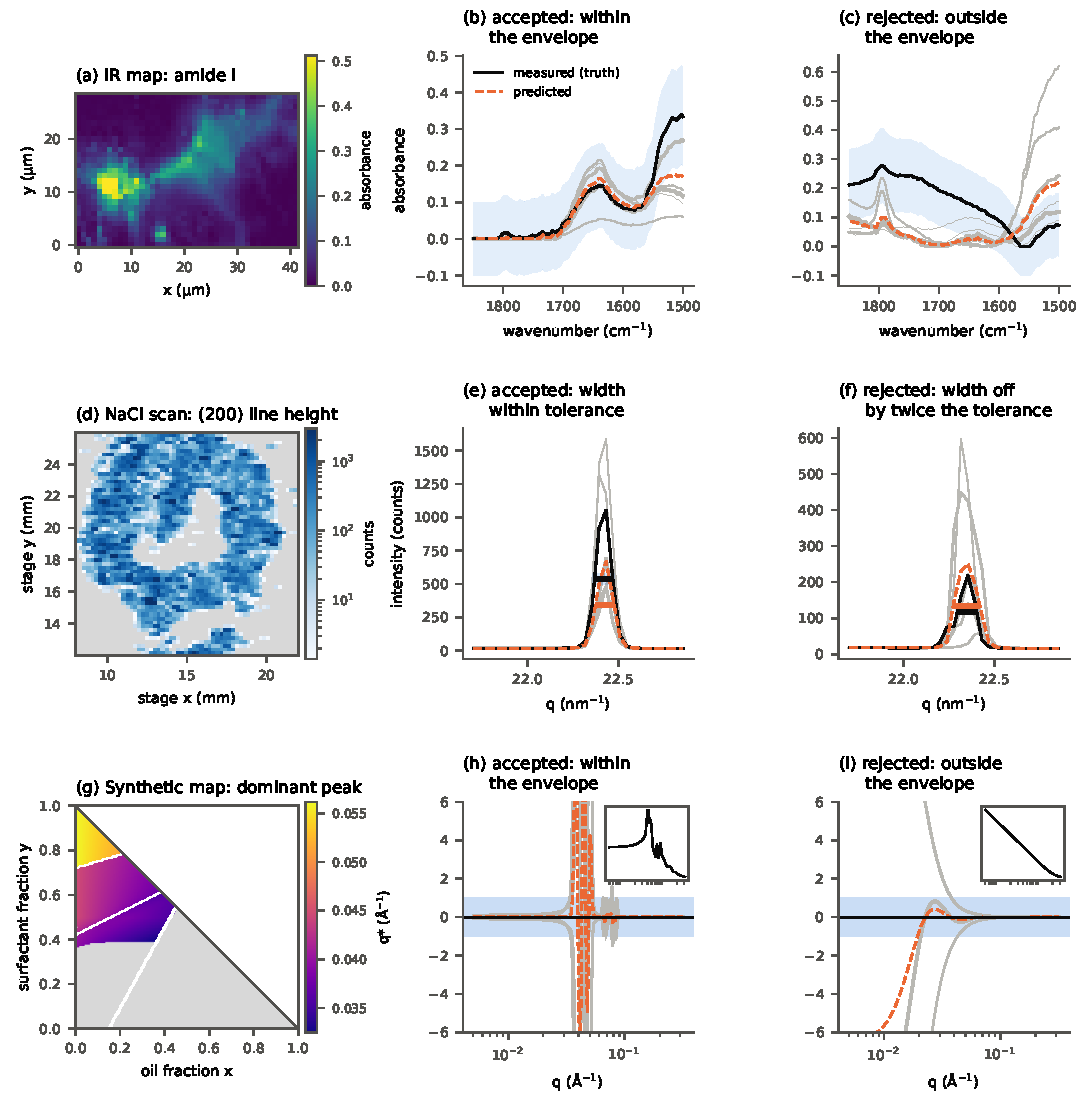
\includegraphics[width=\textwidth,height=0.44\textheight,keepaspectratio]{figures/fig_datasets_claims}
\caption{The three datasets and how their claims judge a prediction; rows: IR map, NaCl scan, synthetic map. Left column, the quantity the claims test: (a) amide-I absorbance, maximum over 1620--1690 cm\ensuremath{^{-1}} after scattering correction, 1 \ensuremath{\mu}m pixels; (d) height of the (200) line where it stands five times the noise above its baseline, grey where absent, the width varying from pixel to pixel by more than the tolerance of the width claim; (g) position of the dominant peak where its prominence reaches 5, grey elsewhere, white lines: phase boundaries of the forward model. Middle and right columns: one site of a guaranteed level that the claim accepts and one it rejects, predicted from the measured sites of the coarser levels by natural-neighbour weights (grey: neighbours, line width by weight; orange: prediction; black: measurement; shaded: tolerance). IR envelope claim: within 10 \% + 0.10 absorbance on average over channels above 0.02. NaCl width claim: widths at half maximum (bars) within 0.02 nm\ensuremath{^{-1}}. Synthetic profile claim, drawn as the deviation of each channel in units of the envelope 0.005 \ensuremath{\times} intensity + 0.005 (shaded: \ensuremath{\pm}1; inset: the measured profile on log--log axes); the claim holds when the mean over channels is at most one, so a few channels near a peak may lie outside.}\label{fig:3}
\end{figure}

\hypertarget{sec:4-2}{%
\subsection{Claims and tolerances}\label{sec:4-2}}

The IR map and the NaCl scan each carry one interest claim and one interpolation claim, fixed before any run. On the synthetic map every site is of interest, and the interpolation claim alone is made, on the full profile.

{\small
\begin{longtable}[]{@{}
  >{\raggedright\arraybackslash}p{(\columnwidth - 4\tabcolsep) * \real{0.3333}}
  >{\raggedright\arraybackslash}p{(\columnwidth - 4\tabcolsep) * \real{0.3333}}
  >{\raggedright\arraybackslash}p{(\columnwidth - 4\tabcolsep) * \real{0.3333}}@{}}
\caption{Claims, fixed before any run.}\label{tab:1}\\

\toprule\noalign{}
\begin{minipage}[b]{\linewidth}\raggedright
Dataset
\end{minipage} & \begin{minipage}[b]{\linewidth}\raggedright
Interest: a site holds
\end{minipage} & \begin{minipage}[b]{\linewidth}\raggedright
Interpolation: the prediction from coarser levels meets
\end{minipage} \\
\midrule\noalign{}
\endhead
\bottomrule\noalign{}
\endlastfoot
Synthetic map & every site (no interest claim) & every point of the profile within 0.5 \% + 0.005, on average over the 240 points \\
NaCl scan & the (200) line at 22.28 nm\ensuremath{^{-1}}, at least five times the noise above its local baseline & the (200) width within 0.02 nm\ensuremath{^{-1}}, the median width difference between neighbouring design sites \\
IR map & absorbance of 0.1 or more in some channel of the window & every channel within 10 \% + 0.10 absorbance, on average over channels above 0.02 \\
\end{longtable}
}

The NaCl tolerance was set from the widths measured over the full scan, without a model of what makes them vary: ten times above the precision of the width and at the median difference between neighbouring design sites (SI 2). A second setting of the IR map tightens the envelope to 10 \% + 0.01, with interest at 0.02 and channels counted above 0.005. Under it, interpolation rather than interest decides the cost. The choice of claim shapes the campaign as much as the budget does; Section~\ref{sec:5-5} and SI 6 compare six metrics on the three datasets.

\hypertarget{sec:4-3}{%
\subsection{Protocols}\label{sec:4-3}}

A protocol pairs a predictor with the scores it supplies, so a difference in cost between protocols reflects both.

\textbf{Natural-neighbour protocol.} Natural-neighbour (Sibson) coordinates \cite{Sibson1981} predict the spectrum at a site as a weighted mean of the measured spectra around it. One set of weights per site serves every channel and every derived quantity. The weights are non-negative and sum to one, so a prediction from non-negative spectra is non-negative. The coordinates are computed exactly by clipping Voronoi cells (SI 1); outside the hull of the measured set, inverse-distance weights over the five nearest measured sites take over.

Both scores are probabilities from logistic regressions fitted on the measured set, the interpolation score on the disagreement between natural neighbours and on position, the interest score on the predicted signal and its spread among the nearest measured sites; on the IR map the interest score is the predicted maximum in the window, capped below the interest level (SI 1). The random scorer of Section~\ref{sec:5-4} assigns every site an independent uniform weight.

\textbf{Gaussian-process protocols.} Gaussian-process regression is the interpolator of choice for autonomous scattering experiments \cite{Noack2019,Noack2020}, and it offers a reason for every measurement: the posterior standard deviation is large where the measured set is far away in units of the length scale. The GP protocols place an isotropic squared-exponential kernel on the coordinates of the hierarchical design and evaluate the process only at design sites \cite{RasmussenWilliams2006}. The posterior mean, clipped at zero because every spectrum here is non-negative, predicts the full spectrum at a site, and the posterior standard deviation at unit output scale orders the sites for the interpolation claim. Both depend on the measured set through one set of linear weights, so the spectrum and any quantity derived from it come from the same fit, as with natural-neighbour coordinates. The interest claim keeps its score from the natural-neighbour protocol, which isolates the change of interpolator.

The length scale is set in three ways, each fixed before the calibration draw of a level: by maximum marginal likelihood on the leading principal-component scores of the measured spectra \cite{Balandat2020}, by the median nearest-neighbour spacing of the design through the finest level measured, or locally, through a Gibbs kernel whose length scale is the distance to the third-nearest measured site \cite{Gibbs1997,PaciorekSchervish2004}. SI 1 gives the details.

\textbf{Common settings.} Levels up to the second form the seed and are measured in full. Every finer level is calibrated on \(m = 40\) sites, or on the whole level when it is smaller. The guarantee on the shared skip-error rate is \(R_E \le 0.10\) at confidence 0.75 on the IR map, \(R_E \le 0.20\) at confidence 0.80 on the NaCl scan and \(R_E \le 0.10\) at confidence 0.80 on the synthetic map. The per-claim form gives each claim half the budget at half the failure probability, so the union bound returns the same statement; with the one claim of the synthetic map the three forms coincide. Every rule uses the exact finite-population tail, and the threshold is placed at the score of the first calibration failure beyond those allowed.

\textbf{Paired comparison (Fig.~\ref{fig:1}).} One question needs model, ranking and calibration sample held fixed: does the model\textquotesingle s own uncertainty, or a threshold set from the calibration sample, keep a rate stated before the round? On the NaCl scan, 80 fresh hierarchical designs over the raster, about 1075 sites each, measure levels up to the third as the seed, about 143 sites, and decide the three finer levels in three rounds of about 135, 268 and 528 sites. Before a round, two Gaussian processes with a squared-exponential kernel, one regressing presence of the (200) line on position and one the logarithm of its width, are fitted on the measured sites and frozen. They give at every site of the round a probability that a skip is wrong, the line predicted present with a width off by more than the tolerance or its presence predicted wrongly, and this probability ranks the sites. A uniform sample of 40 sites is then measured. On the remaining sites both cuts are computed on the identical state, with one target: at most a fifth of the round skipped in error, with probability 0.80. The uncertainty of the model sets the longest prefix of the ranking whose number of skip errors meets the target under 2000 joint draws from the processes, presence drawn site by site and log width jointly from the full predictive covariance. Conformal thresholds set the largest threshold whose exact hypergeometric upper limit from the calibration labels, less the calibration failures already seen, meets the target. One of the two cuts decides which sites are measured and enter the next fit. Three kernels are run: noise level fitted by marginal likelihood; noise fixed at 10\ensuremath{^{-}}\ensuremath{^{4}} of the variance, a common interpolating choice; and noise fixed with the length scale held at 1 mm or more, the assumption that the width varies smoothly at the spacing of the design, where maximum likelihood gives about 0.23 mm. A random predictor replaces the model by a measured site chosen at random for each prediction and by a random ranking; it states nothing about its own errors and runs under the conformal thresholds only. SI 7.4 gives the details.

{\small
\begin{longtable}[]{@{}
  >{\raggedright\arraybackslash}p{(\columnwidth - 2\tabcolsep) * \real{0.5000}}
  >{\raggedright\arraybackslash}p{(\columnwidth - 2\tabcolsep) * \real{0.5000}}@{}}
\caption{Exchangeable parts of a campaign.}\label{tab:2}\\

\toprule\noalign{}
\begin{minipage}[b]{\linewidth}\raggedright
Part
\end{minipage} & \begin{minipage}[b]{\linewidth}\raggedright
Options used
\end{minipage} \\
\midrule\noalign{}
\endhead
\bottomrule\noalign{}
\endlastfoot
Design & Hierarchical Poisson-disk design; seed of levels 0--2; 7 (NaCl, IR) or 9 (synthetic) levels \\
Interpolator & Natural-neighbour coordinates; Gaussian process with length scale by maximum likelihood, by design spacing or by local spacing \\
Interest score & Predicted maximum (IR); logistic on predicted peak height (NaCl); random; none on the synthetic map \\
Interpolation score & Logistic on neighbour disagreement; GP posterior standard deviation; random \\
Form of guarantee & Per-claim budgets; matched-quantile rule; priority rule \\
Calibration & 40 sites per level, uniform without replacement, exact hypergeometric tail \\
\end{longtable}
}

\hypertarget{sec:4-4}{%
\subsection{Evaluation}\label{sec:4-4}}

A guarantee about a probability needs repetition to be checked. Each of 34 configurations was run as 250 campaigns, 20 for the four Gaussian-process configurations of the synthetic map and 50 for one on NaCl, that differ only in their calibration draws and, for the random scorer, in the score stream. Every guaranteed level of every campaign gives one level check against the budget, and the checks over budget are compared with the number expected under the picked failure probabilities (Section~\ref{sec:3-3}). For the first 20 campaigns of each configuration, the calibration draw was also repeated 1000 times on the recorded level populations, which isolates the randomness of the draw (SI 4, SI 5). Four studies extend the record (SI 10): a label-conditional bound, drift, an audit of finished maps and the cost of a plan against its calibration size and confidence.

\hypertarget{sec:5}{%
\section{Results}\label{sec:5}}

All numbers below come from the run record: 34 configurations and nine comparisons, run as 250 campaigns with independent calibration draws, 20 for the four Gaussian-process configurations of the synthetic map and 50 for the process scored by its own probability on NaCl (SI 5).

\hypertarget{sec:5-1}{%
\subsection{The guarantee holds}\label{sec:5-1}}

Checking a probability bound needs repeated campaigns against a known truth. Every guaranteed level of every campaign was therefore checked against the fully measured truth (SI 5).

The picked failure probabilities \(\delta_L\) (Section~\ref{sec:3-3}) averaged 0.19 against a nominal 0.25 for the IR map, 0.12 against 0.20 for the NaCl scan and 0.10 against 0.20 for the synthetic map. The observed exceedances are to be compared with \(\delta_L\), and the four levels of a NaCl campaign hold together with probability at least about one half.

The record agrees with the guarantee at the picked failure probabilities: over the 25 statements of 250 campaigns whose budget can be exceeded on every level, observed exceedances lay between 0.88 and 1.11 times the number expected, between 0.67 and 1.14 for the five Gaussian-process rows of 20 or 50 campaigns, and none exceeded it beyond chance (SI 5, Table S5.3). On the IR map at its original tolerance, three of the four levels hold too few failing sites for the budget to be reached. Repeating the calibration draw on the recorded level populations gives the same picture (Table S5.2). Against a fixed truth these counts check the rule and its implementation (Section~\ref{sec:6}).

A plan can be guaranteed for all levels together by dividing its failure probability among its levels when it is declared. Guaranteed level by level, the plans exceeded the budget on at least one level in 20 \%, 38 \% and 46 \% of campaigns on the IR, NaCl and synthetic maps. Guaranteed for all levels together, at confidence 0.75 for IR and 0.80 for the other two, they measured 415 \ensuremath{\pm} 82, 694 \ensuremath{\pm} 58 and 1189 \ensuremath{\pm} 286 sites, 41 \%, 13 \% and 28 \% more, and exceeded it in 1, 24 and 16 of 250 campaigns, within the 25 \% and 20 \% the specifications allow (SI 5.3). Their 1, 27 and 16 level checks over budget compare with 30, 28 and 13 expected under the picked failure probabilities.

Conformal risk control on the same draw bounds the expected share of a level skipped in error, averaged over draws, in place of a PAC bound \cite{Angelopoulos2024}. It measured 260, 542 and 673 sites. Its mean share of a level skipped in error, 5.7 \%, 18.8 \% and 8.8 \%, stayed below the budget, as promised; single levels exceeded it in 5 \%, 35 \% and 32 \% of checks, and campaigns on at least one level in 20 \%, 81 \% and 90 \% (SI 5.3).

Table~\ref{tab:3} gives one configuration per map: what was measured, why each site was skipped, and how the record compares with the guarantee. The guarantee bounds skip errors as a share of all sites of a level; among the skipped sites alone the share is larger, up to 26.7 \% on the NaCl scan.

{\small
\begin{longtable}[]{@{}
  >{\raggedright\arraybackslash}p{(\columnwidth - 12\tabcolsep) * \real{0.1429}}
  >{\raggedright\arraybackslash}p{(\columnwidth - 12\tabcolsep) * \real{0.1429}}
  >{\raggedright\arraybackslash}p{(\columnwidth - 12\tabcolsep) * \real{0.1429}}
  >{\raggedright\arraybackslash}p{(\columnwidth - 12\tabcolsep) * \real{0.1429}}
  >{\raggedright\arraybackslash}p{(\columnwidth - 12\tabcolsep) * \real{0.1429}}
  >{\raggedright\arraybackslash}p{(\columnwidth - 12\tabcolsep) * \real{0.1429}}
  >{\raggedright\arraybackslash}p{(\columnwidth - 12\tabcolsep) * \real{0.1429}}@{}}
\caption{One guarantee per dataset: matched-quantile rule, natural-neighbour interpolation, 250 campaigns; counts are means per campaign. Skip errors are given as a share of the sites on guaranteed levels, the quantity the guarantee bounds, and as a share of the skipped sites. Expected exceedances are the sums of the picked failure probabilities over the level checks.}\label{tab:3}\\

\toprule\noalign{}
\begin{minipage}[b]{\linewidth}\raggedright
Dataset
\end{minipage} & \begin{minipage}[b]{\linewidth}\raggedright
Guarantee
\end{minipage} & \begin{minipage}[b]{\linewidth}\raggedright
Sites
\end{minipage} & \begin{minipage}[b]{\linewidth}\raggedright
Measured: seed / calibration / no claim
\end{minipage} & \begin{minipage}[b]{\linewidth}\raggedright
Skipped: not of interest / predictable / both
\end{minipage} & \begin{minipage}[b]{\linewidth}\raggedright
Skip errors: count (share of sites / of skips)
\end{minipage} & \begin{minipage}[b]{\linewidth}\raggedright
Exceedances: observed / expected
\end{minipage} \\
\midrule\noalign{}
\endhead
\bottomrule\noalign{}
\endlastfoot
IR map & \(R_E \le 0.10\) at 0.75 & 959 & 73 / 160 / 62 & 37 / 228 / 399 & 34 (3.8 \% / 5.1 \%) & 49 / 190; reachable levels 49 / 56 \\
IR map, tight tolerance & \(R_E \le 0.10\) at 0.75 & 959 & 73 / 160 / 388 & 8 / 257 / 73 & 54 (6.1 \% / 15.9 \%) & 193 / 190 \\
NaCl scan & \(R_E \le 0.20\) at 0.80 & 1071 & 76 / 160 / 378 & 157 / 156 / 144 & 122 (12.3 \% / 26.7 \%) & 112 / 120 \\
Synthetic map & \(R_E \le 0.10\) at 0.80 & 2118 & 39 / 233 / 660 & -- / 1186 / -- & 98 (4.7 \% / 8.2 \%) & 147 / 143 \\
\end{longtable}
}

Breaking the order of operations breaks the guarantee (Section~\ref{sec:3-1}). On a simulated level of 399 sites with a budget of 0.10 and a picked failure probability of 0.206, the calibration draw was repeated 4000 times under several rules (SI 5.2). Scores frozen before a uniform draw exceeded the budget in 20.5 \% of draws, as did a score that knew the true labels: what the score knows changes the cost and leaves the guarantee intact. Rules that use the draw broke it, in every draw when the scores of failing calibration sites were raised afterwards, in 63 \% when calibration sites were taken where the scores were least sure, as an active learner would, and in 69 \% when the best of five draws was kept. Setting one threshold on the calibration sites the other left uncovered exceeded the budget in 28.8 \% of draws, where the priority rule, which fixes the same preference in advance, stayed at 20.5 \%. Every form of Table S4.3 kept its guarantee, and none was the least expensive on all three maps (Fig. S3; Table S3.1).

\hypertarget{sec:5-2}{%
\subsection{What the model states about itself}\label{sec:5-2}}

Decisions resting on a model\textquotesingle s stated error rate need that rate to hold. Held to one target, at most a fifth of each round skipped in error with probability 0.80, the two cuts of the paired comparison behaved differently (Fig.~\ref{fig:1}; Section~\ref{sec:4-3}). With the noise level fitted, the Gaussian process kept its stated rate in 88 \%, 99 \% and 100 \% of 80 campaigns over the three rounds and measured 543 sites; the noise term took up the scatter of the width between neighbouring sites, so the statement was cautious. With the noise fixed at 10\ensuremath{^{-}}\ensuremath{^{4}} of the variance it kept the rate in 74 \%, 69 \% and 89 \% of campaigns at 500 sites, and with the length scale held at 1 mm or more in none, at 317 sites, skipping in error about 31 \%, 38 \% and 39 \% of each round against a stated fifth. Conformal thresholds set from the same calibration samples kept the rate in 78 \%, 84 \% and 83 \% of campaigns with the noise level fitted, 83 \%, 89 \% and 89 \% with the noise fixed and 88 \%, 81 \% and 78 \% with the long length scale, at 580, 619 and 723 sites; a method meeting the target exactly keeps it in 71 \% to 89 \% of 80 campaigns, 95 times in 100. Both cuts were computed on every state, so the comparison also holds within a campaign: driven by the model\textquotesingle s cut, the thresholds kept the rate in 78 \%, 85 \% and 81 \% of campaigns with the noise level fitted, 83 \%, 81 \% and 89 \% with the noise fixed and 88 \%, 78 \% and 84 \% with the long length scale (SI 7.4).

The measurements a poor model is made to take improve the map. Each measured set was refitted with one Gaussian process, a Matérn kernel of smoothness ½ with fitted noise for presence and width, and the map compared with the full raster of 3249 sites (SI 7.4). Over 20 designs, the sites measured under conformal thresholds with the long length scale left 24.0 \% of the raster outside tolerance, against 29.9 \% for the sites chosen by the model\textquotesingle s own uncertainty, and the thresholds gave the better map in all 20 (Wilcoxon signed-rank \(p = 2 \times 10^{-6}\)); presence alone was wrong at 4.7 \% against 7.7 \% of the raster. Random sets of the same sizes left 25.3 \% and 30.5 \%, so the gain came from the number of sites measured. With the noise level fitted, the two maps were equal, 26.0 \% against 25.9 \%. Measuring every site of one design left 19 \% of the raster outside tolerance, since the width varies between neighbouring raster sites by about the tolerance.

Other statements of the same kind lead to the same conclusion. On the NaCl scan, a Gaussian process refitted after each level of the same fixed design skipped a site when it was sure the line was absent, or when its 68 \% interval on the width, from the predictive standard deviation, lay within the tolerance (SI 7). Its statement, the model\textquotesingle s own probability of a skip error summed over its skips, can be set against the realised share of the level, the quantity the guarantee bounds. The fitted noise took about three quarters of the variance of the width, the site-to-site scatter of the sample, so no interval fell within the tolerance; every skip was for want of a line, and the process stated 0.4 \% and realised 0.3 \%, at 922 measurements. The comparison can also hold model and ranking fixed. With the process of Section~\ref{sec:4-3} as predictor and its own posterior probability of a skip error as the frozen score, a guaranteed plan measured 761 \ensuremath{\pm} 68 of 1071 sites over 50 campaigns and exceeded the budget on 16 of 200 level checks, against 24 expected; skipping where that same probability was at most \ensuremath{\alpha}, for \ensuremath{\alpha} from 0.01 to 0.32, the process measured 1064 to 1070 (Fig. S7b). The guaranteed plans measured 614 \ensuremath{\pm} 56 sites with natural-neighbour interpolation and 745 to 777 with the Gaussian process as predictor, and their bound held at the stated confidence (Fig. S7). With model and score held fixed, the guaranteed plan skipped sites that the process\textquotesingle s own statements withheld: 761 measurements, against 922 under its 68 \% interval and 1064 to 1070 under its own probability.

The comparison was repeated on all three maps with the Gaussian process of the guaranteed campaigns in Section~\ref{sec:5-4}, which predicts the whole profile. A site was skipped under a claim when the posterior probability of a skip error was at most \ensuremath{\alpha}, for \ensuremath{\alpha} from 0.01 to 0.32, with the predictive standard deviation or with that deviation rescaled to the leave-one-out residuals of the measured sites (SI 7). On the synthetic map, under the profile claim, the process judged every site too uncertain to skip at every \ensuremath{\alpha} and measured all 2118; a guaranteed plan with the same process and score measured 1991 \ensuremath{\pm} 91 over 20 campaigns. Its mean prediction failed at 77 \% of the calibration sites, against 40 \% for natural-neighbour prediction, which measured 932 \ensuremath{\pm} 223. Rescaled to the leave-one-out residuals, it measured 1506 to 1792 sites, stated 0 \% to 1.8 \% and realised 0.3 \% to 2.1 \%; the scale fell to between 0.06 and 0.23 of its value, because the sites the process chose to measure were easier for it to predict than those it left out, the bias a uniform draw removes. On IR the stated shares stayed below 10 \% and the realised ones below 5 \%, with 73 to 398 of 959 sites measured. On NaCl the process judged almost every site too uncertain to skip and measured 959 to 1070 of 1071 (Fig.~\ref{fig:4}).

A rate stated by the model can thus be right, too low, or so cautious that nothing is skipped, and only sites the model did not choose show which (Section~\ref{sec:5-6}). The guaranteed campaigns at budgets from 0.05 to 0.30 realised on average less than their bound on every map; points from guaranteed campaigns pair a bound with a mean, and points from campaigns without a guarantee a stated expectation with a realisation.

\begin{figure}[tbp]
\centering
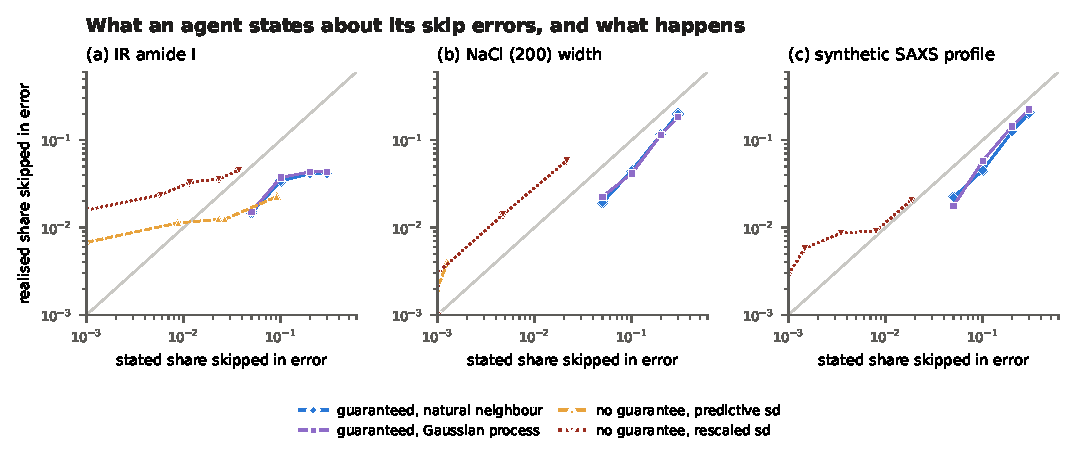
\includegraphics[width=\textwidth,height=0.44\textheight,keepaspectratio]{figures/fig_stated}
\caption{What an agent states about its skip errors, and what happens. Stated against realised share of sites on guaranteed levels skipped in error, for guaranteed campaigns with natural-neighbour (blue) and Gaussian-process (purple) prediction at budgets 0.05 to 0.30 (the bound against the mean over 20, or 8 for the Gaussian process, 4 on the synthetic map) and for Gaussian-process campaigns without a guarantee at \ensuremath{\alpha} from 0.01 to 0.32 with predictive or rescaled standard deviation; shares below 10\ensuremath{^{-}}\ensuremath{^{3}} are drawn at 10\ensuremath{^{-}}\ensuremath{^{3}}; grey: equality.}\label{fig:4}
\end{figure}

\hypertarget{sec:5-3}{%
\subsection{A reason for every site}\label{sec:5-3}}

An instrument record becomes useful once every site of a map carries its reason. Figure~\ref{fig:5} shows one campaign of average cost per dataset under the matched-quantile rule with natural-neighbour interpolation, with every design site marked by the reason recorded for it and every skip error found against the fully measured truth.

In the campaigns shown, the skip errors were 3.8 \% of the sites on guaranteed levels of the IR map, against a budget of 0.10 per level, 11.8 \% on NaCl, against 0.20, and 5.3 \% on the synthetic map, against 0.10. The skip errors of the synthetic map gather along the phase boundaries and the walls of the composition triangle; the guarantee bounds their rate on each level and leaves their location open (Section~\ref{sec:5-5}; SI 6).

In hindsight, the record shows which measurements every claim would have skipped in error (SI 8): 43 \% of the sites measured for want of a claim on the synthetic map, against 40 \% of sites drawn at random, where the tight tolerance fails at most sites, and 47 \% against 35 \% on NaCl, where the width varies between neighbouring sites by about the tolerance.

\begin{figure}[tbp]
\centering
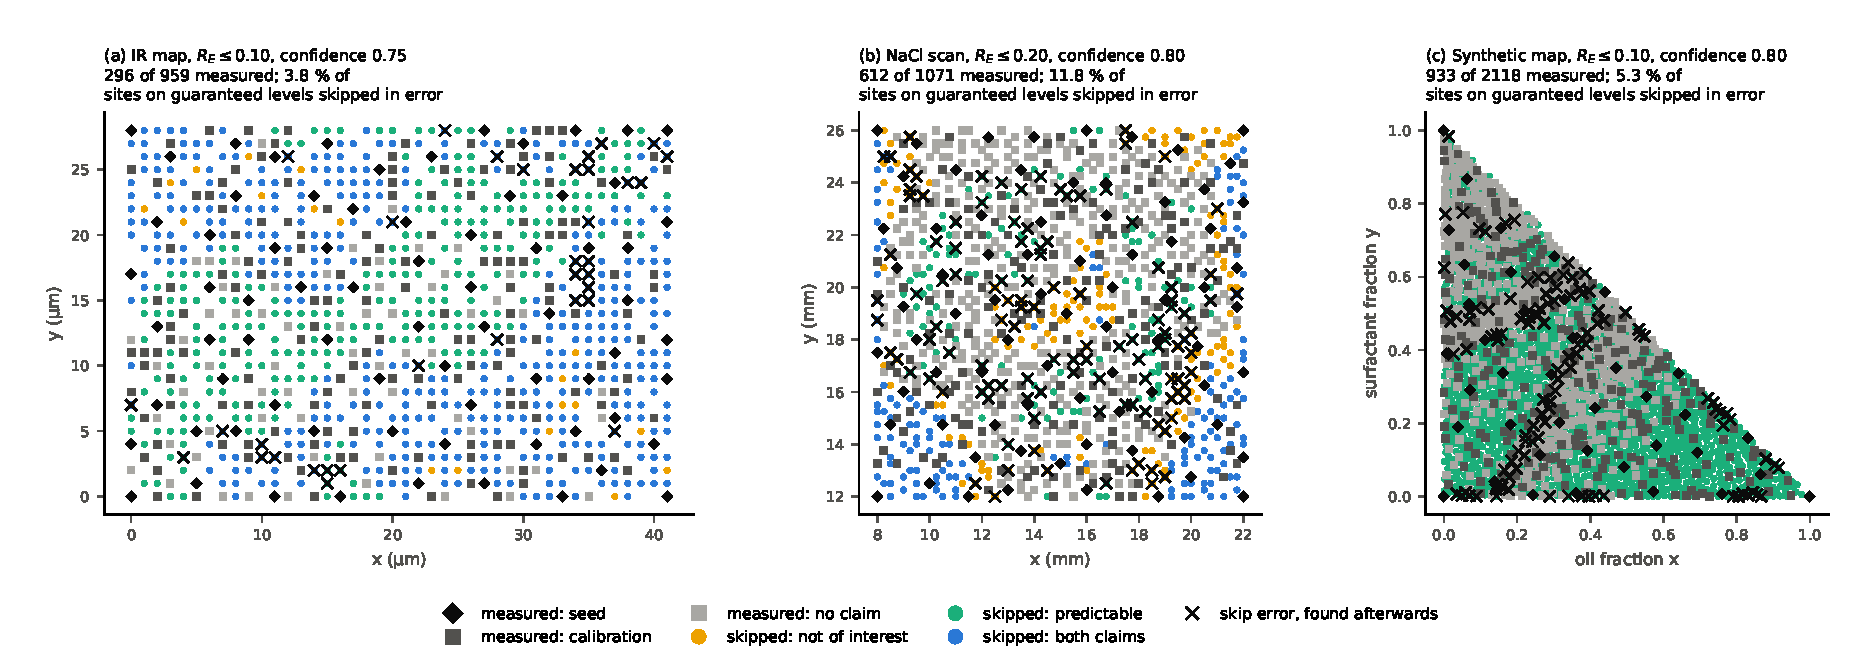
\includegraphics[width=\textwidth,height=0.44\textheight,keepaspectratio]{figures/fig5_maps}
\caption{Maps with reasons, one campaign of average cost per dataset (matched-quantile rule, natural-neighbour interpolation; NaCl: random state 44; the same campaigns as SI 8). Measured sites: seed (black diamonds), calibration (dark grey squares) and sites without a claim (light grey squares). Skipped sites: not of interest (yellow), predictable (green) and both (blue). Crosses: skip errors against the fully measured truth. IR in micrometres, NaCl in stage millimetres, synthetic map in composition fractions.}\label{fig:5}
\end{figure}

\hypertarget{sec:5-4}{%
\subsection{Cost under different models}\label{sec:5-4}}

Any model may supply predictor and score, and its choice sets the number of measurements. The matched-quantile rule was run with four interpolation protocols on each dataset at the nominal guarantees of Section~\ref{sec:5-1}: natural-neighbour interpolation with the logistic score, and Gaussian-process interpolation with the posterior standard deviation as score and three rules for the length scale (Section~\ref{sec:4-3}). At the original IR tolerance almost every site is interpolable and the interest claim alone sets the cost; at the tight tolerance interpolation decides.

A score that carries no information still yields a valid guarantee, at a price. A random scorer, an independent uniform weight per site and claim, exceeded the budget no more often than expected on every map and cost 1.4 to 2.4 times as many measurements as informed scores, 716 \ensuremath{\pm} 71 against 295 \ensuremath{\pm} 53 of 959 sites on IR (Fig.~\ref{fig:6}). A predictor without information fares the same. The random predictor of Fig.~\ref{fig:1}, which copies a measured site chosen at random and ranks at random, would have skipped in error 69 \% of each round had it skipped everything; under conformal thresholds it kept the stated rate in 80 \%, 79 \% and 83 \% of 80 campaigns and measured 891 of about 1075 design sites, against 580 to 723 with the Gaussian processes. The guarantee comes from the calibration draw; the score decides what it costs.

Every guarantee held, with exceedance counts on each map close to those expected under the picked failure probabilities and none beyond chance (Fig.~\ref{fig:6}; Table S5.3).

The cost depends on the protocol and on the data (Fig.~\ref{fig:6}; Table S3.2). At the original IR tolerance the four protocols measured 273 \ensuremath{\pm} 31 to 295 \ensuremath{\pm} 53 of 959 sites with skipped sets overlapping by about 90 \%; at the tight tolerance they measured 621 \ensuremath{\pm} 70 to 799 \ensuremath{\pm} 40, and the Gaussian-process protocols shared a quarter to a third of their skips with natural-neighbour interpolation. On NaCl, the Gaussian-process protocols measured 745 to 777 of 1071 sites, against 614 \ensuremath{\pm} 56. On the synthetic map they measured between 1946 \ensuremath{\pm} 50 and 2027 \ensuremath{\pm} 39 of 2118 sites over 20 campaigns each, against 932 \ensuremath{\pm} 223 with natural-neighbour interpolation and 1578 \ensuremath{\pm} 248 with random scores; their score, the posterior standard deviation at unit output scale, depends on the positions of the measured sites and the length scale only. Ranking by the process\textquotesingle s own probability of a skip error instead measured 761 \ensuremath{\pm} 68 on NaCl and 1991 \ensuremath{\pm} 91 on the synthetic map, no fewer. The difference arises in the calibration draws: more failing calibration sites admit fewer skips at the same budget, and the guarantee is unchanged.

A guaranteed plan is worth its calibration samples only if it does better than a uniform sample of the same size. With every other site predicted from all measured sites, such a sample left 0.5 \ensuremath{\pm} 0.2 \%, 22.0 \ensuremath{\pm} 1.0 \% and 10.4 \ensuremath{\pm} 0.7 \% of the sites on guaranteed levels outside tolerance on the IR, NaCl and synthetic maps; the final maps of the guaranteed plans, predicted in the same way, left 0.4 \ensuremath{\pm} 0.3 \%, 18.0 \ensuremath{\pm} 3.8 \% and 3.6 \ensuremath{\pm} 1.8 \% (SI 5.3). The specification sets the rest: on the IR map at confidence 0.80, calibration samples of 20, 40 and 80 sites per level cost 340 \ensuremath{\pm} 90, 337 \ensuremath{\pm} 63 and 393 \ensuremath{\pm} 22 measurements, and at 0.95 a sample of 20 supported a guarantee on no level (SI 10.4).

\begin{figure}[tbp]
\centering
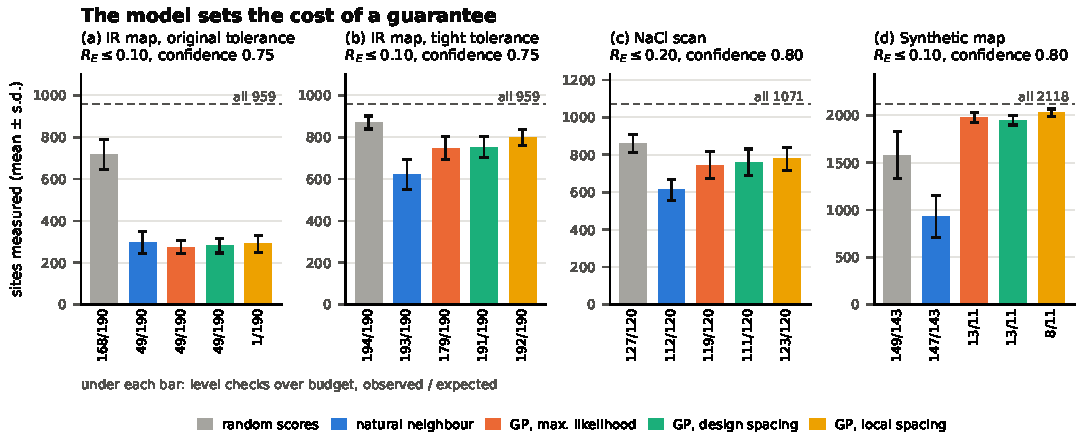
\includegraphics[width=\textwidth,height=0.44\textheight,keepaspectratio]{figures/fig_cost}
\caption{What a guarantee costs under different models: sites measured (mean \ensuremath{\pm} s.d. over 250 campaigns, matched-quantile rule) with random scores and with four interpolation protocols, against the number of design sites (dashed). Under each bar: level checks over budget on the shared rate, observed against expected under the picked failure probabilities. GP: Gaussian process with isotropic squared-exponential kernel; length scale by maximum likelihood, by design spacing, or by local spacing of measured sites.}\label{fig:6}
\end{figure}

\hypertarget{sec:5-5}{%
\subsection{What each claim protects}\label{sec:5-5}}

Each claim protects what it states, so its choice deserves a record. Six acceptance metrics were compared on the three maps with the interpolation claim alone (SI 6). Every metric kept its guarantee, and the metric set the cost: at tolerances a practitioner might pick, the IR map needed between 233 and 810 measurements. At tolerances matched to equal difficulty the metric still decided where measurements went, with the peak claim on the synthetic map measuring where the peak drifts with composition and the profile claim along the phase boundaries (Fig. S6), and it decided where skip errors fell. The rate counts skip errors over all sites of a level. On a variant of the synthetic map that adds an interest claim, a dominant peak at least five times its baseline, to a claim on the peak position and width at a budget of 0.20, a third of the sites are of interest, and 35 \% of them on guaranteed levels were skipped in error while every level met its budget (SI 6.2).

The label-conditional statement of Section~\ref{sec:3-4} closes that gap. On that variant, at a share of 0.20 and confidence 0.80, calibrated on 12 to 20 sites of interest per level, the plan lost 8.5 \ensuremath{\pm} 4.4 \% of the interesting sites, against 34.7 \ensuremath{\pm} 8.5 \%, at 359 \ensuremath{\pm} 26 measurements against 334 \ensuremath{\pm} 26; 4.9 \% of level checks exceeded the share, below the 20 \% that confidence 0.80 allows, because few sites of interest make the allowed number of failures coarse; without the statement, 58.7 \% of levels lost more than that share. On NaCl, where two thirds of the sites hold the line, the shared budget already spared them, and the statement changed the share lost from 9.2 \% to 8.1 \% at 16 more measurements (SI 10.1).

\hypertarget{sec:5-6}{%
\subsection{Checks on the finished map}\label{sec:5-6}}

An audit of 100 skipped sites after the last level (Section~\ref{sec:3-6}) bounded, at confidence 0.80, the share of sites on guaranteed levels that the final map predicts outside tolerance at 1.5 \% on average, 19.8 \% and 5.1 \% on the IR, NaCl and synthetic maps, against 0.4 \%, 18.0 \% and 3.6 \%, and held in 100 \%, 83 \% and 86 \% of audit draws (SI 10.3). A campaign steered by its own model meets a budget when the model\textquotesingle s statement holds, and learns whether it held only afterwards. On the NaCl scan a Gaussian process measured, batch by batch, the sites at which it judged a skip most likely to be wrong, and stopped once its stated share of sites on guaranteed levels predicted wrongly reached 0.20 (SI 10.3). In 30 runs it stopped after 451 to 501 measurements with 14.6 \ensuremath{\pm} 0.6 \% of the sites wrong, because its fitted noise made the statement conservative on this scan; on the synthetic map the same kind of statement, rescaled to the leave-one-out residuals, was up to four times too low (Section~\ref{sec:5-2}). The guaranteed plan with the same process as predictor and score measured 761 \ensuremath{\pm} 68 sites, the price, on this scan, of a bound known before each level was decided (Fig. S7b). An audit of 100 sites at the stopping point, the first check open to a real run, confirmed the budget in 89 \% of draws.

Drift was simulated as a slow swelling of the synthetic sample, its \(q\) scale stretched in proportion to the number of sites measured before, by 5 \% to 20 \% over the mean cost of the plan (SI 10.2). Under the profile claim the bound broke: at a stretch of 5 \% the levels exceeded their budget in 24 \% of checks against 9.5 \% expected, the plan measured 1687 \ensuremath{\pm} 76 sites against 966 \ensuremath{\pm} 247, and 88 \% of the measurements lay outside tolerance of the sample at the start, where no claim applies. Five seed sites measured again after each level flagged every drifted campaign from the fourth level on, and none without drift.

\hypertarget{sec:6}{%
\section{Discussion}\label{sec:6}}

A policy fixed before a campaign is worth as much as the campaign's adherence to it. Conformal thresholds force that adherence: the stated rate holds as often as promised, whatever the model, and the model sets only how many measurements adherence costs (Fig.~\ref{fig:1}).

\hypertarget{what-the-specification-costs}{%
\subsection{What the specification costs}\label{what-the-specification-costs}}

A bound is worth most when it is known at the moment a decision rests on it. Two simpler routes give a statement about a campaign: a uniform sample of the same size, or a model steering on its own uncertainty, each followed by an audit of the finished map. Both report once every skip has been made, and a skip found wrong then is a site that can rarely be measured again. The specification moves the statement to the decision, and it charges for the move in measurements. Calibration costs 40 sites on each guaranteed level, up to a sixth of the IR map, a share that falls as maps grow, since the budget and the confidence alone set the sample size. A plan guaranteed for all levels together cost 13 \% to 41 \% more than a plan guaranteed level by level (Section~\ref{sec:5-1}). With model, ranking and calibration sample held fixed on the NaCl scan, conformal thresholds measured 580 to 723 sites where the uncertainty of the model measured 317 to 543, and only the thresholds kept the stated rate with every kernel (Section~\ref{sec:5-2}). The cost is in measurements alone: the final maps of the guaranteed plans left no more sites outside tolerance than a uniform sample of the same size, and on the synthetic map a third as many (Section~\ref{sec:5-4}). The record adds a second value in failure. A level over budget is either chance at the stated rate or a sign that a condition of Section~\ref{sec:3-1} failed, through drift, beam damage or a draw that was not uniform; seed sites measured again after each level expose drift (Section~\ref{sec:5-6}), and the specification states in advance what a flag stops. An agent without a guarantee leaves its errors unapportioned between model, data and chance.

\hypertarget{choice-of-model}{%
\subsection{Choice of model}\label{choice-of-model}}

The bound concerns a decision, and it holds whatever model proposes the skips. A model steering a campaign selects the sites on which it would be judged, so a check run on them is circular \cite{Kriegeskorte2009}. A coherent Bayesian forecaster gives probability one to its own long-run calibration \cite{Dawid1982}, so the check has to come from outside the model. Intervals built by cross-validation, such as the jackknife+ \cite{Barber2021}, need the measured sites to be exchangeable with the skipped ones, and selection by the model breaks that unless the selection probabilities are known \cite{Fannjiang2022,ZrnicCandes2024}; on the synthetic map rescaling to leave-one-out residuals shrank the stated uncertainty, because the measured sites were easier to predict than the skipped ones (Section~\ref{sec:5-2}). A better kernel may make a process honest on a given map, and whether it did is again known only afterwards; the specification makes the question moot for the guarantee and leaves it to the cost. A uniform sample drawn before the decision turns the check into a bound, through the order statistic of Section~\ref{sec:3-3}, at no cost beyond the calibration sample of the plan. Any kernel then enters as predictor and score, and the quality of its predictions returns as fewer measurements: under the conformal thresholds of Fig.~\ref{fig:1}, the processes measured 580 to 723 of about 1075 sites and the random predictor 891, all at the stated rate (Sections 5.2, 5.4). Ranking by the process\textquotesingle s own probability of a skip error saved none over its positional uncertainty (Section~\ref{sec:5-4}). The process used here serves as an illustration, and what it did on these maps concerns this process alone.

\hypertarget{scope-of-the-guarantee}{%
\subsection{Scope of the guarantee}\label{scope-of-the-guarantee}}

A map built under a guarantee serves its reader to the extent that the reader knows what the bound covers. The bound concerns the share of skip errors among all design sites of a level, with probability over the calibration draw. Section~\ref{sec:5-5} and SI 6 show the two consequences: skip errors gather in space, and when signal is rare a budget met on every level can still cost a large share of the sites of interest. A label-conditional statement bounds the share of interesting sites lost (Section~\ref{sec:5-5}); it rests on the calibration sites of interest alone, so a rare signal calls for a larger draw. Labels compare with one measurement (Section~\ref{sec:3-5}). On the NaCl scan the width of the line varies across the sample at the scale of the tolerance, so about half of all predictions fail whatever the model, while counting noise moves the width far less (SI 2); the variation is structure in the sample, from strain, crystallite size or orientation, and measuring most sites is the correct outcome for a claim at that tolerance. Fully measured data check the rule against a fixed truth, and the 250 campaigns per configuration check its implementation. A live campaign remains untested: simulated drift broke the bound and moved most of the error into the measurements, where repeated seed sites found it (Section~\ref{sec:5-6}), and a drift so found can be modelled from the repeated sites and removed, or the calibration sites weighted by age at a bounded loss of coverage \cite{Barber2023}; a measurement that disturbs its neighbours remains a question for the instrument.

\hypertarget{choice-of-claim}{%
\subsection{Choice of claim}\label{choice-of-claim}}

A guarantee is stated for one acceptance metric, and the metric deserves the same care as the budget. The bound holds for any metric fixed before the calibration draw, and the metric decides the rest: which sites fail prediction, where measurements are taken and where skip errors gather (Section~\ref{sec:5-5}). The same holds for any autonomous experiment: the quantity a model predicts, and the error its acquisition anticipates, decide where measurements are taken \cite{Noack2019,Noack2020}. The guarantee delivers the claim as specified, and features outside that claim carry no protection. The metric is therefore best fixed from the scientific question before beam time, written into the specification, and checked on a pilot scan for the cost it implies.

\hypertarget{extensions}{%
\subsection{Extensions}\label{extensions}}

An audit sits over any campaign, whatever its rule, at the cost of its sample (Section~\ref{sec:5-6}). A guarantee on each level sits over any campaign that fixes its proposals for a level before its draw: the proposals of an acquisition-driven Gaussian process enter as a frozen score, and within an action the remaining sites can follow the shortest path of the instrument. Costs here are counted in sites; at an instrument each level adds a second pass, the calibration sample measured and reduced before the rest is decided, and a fast raster of the whole plan may compete with scattered single measurements. Any rate that counts sites can be bounded, and ratios such as the share of skips that are wrong are controlled through conformal p-values \cite{Jin2023}. Two conditions carry every such statement: the calibration sites are an exchangeable draw from the population the statement concerns, a Mondrian category fixed before the draw taking the place of the level \cite{Vovk2005}, and the rule is non-anticipating (Section~\ref{sec:3-1}). For a bounded loss graded by the size of an error, confidence sequences for sampling without replacement \cite{WaudbySmith2020} give a bound of the same kind and would let calibration stop as soon as the bound is settled. The design needs only a fixed plan, a claim that can be checked by measuring and a uniform draw, so it applies beyond the beamline, to autonomous synthesis, to campaigns of electronic-structure calculations and to agents that choose which computations to run. Optimisation is the natural next case; reweighting by the known selection mechanism \cite{Tibshirani2019,Fannjiang2022,Barber2023}, online control of a long-run rate \cite{Gibbs2021} and level sets, each a mapping problem with a threshold fixed before its draw \cite{CerouGuyader2007,Gotovos2013}, offer routes to a bound.

\hypertarget{accountable-experiments}{%
\subsection{Accountable experiments}\label{accountable-experiments}}

An accountable experiment fixes its specification before the first measurement and attaches a bound to every decision before the decision is taken. The workflow leaves both in its record. Each site carries its level, scores and reason; each level carries its calibration draw, picked failure probability, thresholds and bound. The guarantee rests on the order of operations, so the record suffices: predictor and scores are frozen and recorded before each draw, the draw is reproduced from its recorded random state, and every decision can be replayed, every bound recomputed (SI 5) and every measurement checked in hindsight (SI 8). Claims, tolerances and budgets form the specification and remain the experimenter\textquotesingle s choice; the record shows that the specification was kept, and the audit reports how well the finished map holds.

\hypertarget{sec:7}{%
\section{Conclusion}\label{sec:7}}

An autonomous experiment decides where not to measure, and each such decision needs a bound when it is taken. The model steering the campaign cannot give one: it estimates its error on the sites it selected, and a coherent model is sure of its own calibration. A specification fixed before the campaign breaks that cycle. It names the plan, the claims under which a site may be skipped, and a budget on skip errors with its confidence. On each level of the plan one decision is taken, after a uniform draw from a level fixed before it, and a PAC bound on that decision, a share skipped in error below the budget at least as often as the stated confidence, is known before any of its sites is skipped; the order fit, freeze, draw, calibrate, decide keeps each draw exchangeable with its level whatever came before, so the bound holds for any model. On three fully measured datasets the record matched the guarantees, with informed and random scores and with natural-neighbour and Gaussian-process prediction. The model set the cost, and knowing the bound in advance was paid for in measurements, up to 41 \% for a plan guaranteed on all levels together. The claim decided what a guarantee bought, so the claim belongs to the scientific question and enters the specification with it. A held-out audit bounded the error of the finished map for any campaign. Deployment at autonomous instruments, beginning with a synthesis campaign, optimisation through level sets and a model of beam time are the next steps, and the specification carries over to any campaign in which a model chooses what to evaluate and what to leave out, among them screens of electronic-structure calculations and agents that choose which computations to run. Each skipped site leaves the campaign with a reason and a claim, each level with a PAC bound fixed before its decision, and the record allows every decision to be replayed.


\appendix
\hypertarget{app:A}{%
\section{Exchangeability by design and the single-claim bound}\label{app:A}}

\hypertarget{conditions}{%
\subsection{Conditions}\label{conditions}}

A campaign processes the levels \(L = L_s + 1, L_s + 2, \dots\) of a hierarchical design in order. Write \(\mathcal{F}_{L-1}\) for everything known before the calibration draw of level \(L\): the design, the sites measured so far and their spectra, all earlier calibration draws, and any auxiliary randomness used by the scores. The truth \(y(x)\) at every design site is fixed; for a live experiment, \(y(x)\) is the outcome a measurement of \(x\) would return.

The order of operations of Section~\ref{sec:3-1} amounts to six conditions.

\begin{itemize}
\tightlist
\item
  \textbf{(A1) Fixed population.} The level population \(D_L\), of size \(N_L\), is determined by \(\mathcal{F}_{L-1}\). It may be declared before the experiment or drawn up from the sites measured so far; in this work the plan is declared in full before the experiment.
\item
  \textbf{(A2) Frozen scores and predictor.} The scores \(S_j\) and the predictor \(\hat y_L\) on \(D_L\) are determined by \(\mathcal{F}_{L-1}\).
\item
  \textbf{(A3) Labels.} Each bad label \(B_j(x)\), \(x \in D_L\), is a fixed function of the truth and of \(\hat y_L\), so the labels of the whole level are determined given \(\mathcal{F}_{L-1}\), whether or not a site is drawn.
\item
  \textbf{(A4) Fixed rule.} The family of covers searched (thresholds on one score, a path, a split of the budget), the budget \(\varepsilon\), the failure probability \(\delta\), the sample size \(m\) and the allowed number of failures \(k\) are determined by \(\mathcal{F}_{L-1}\).
\item
  \textbf{(A5) Uniform draw.} Given \(\mathcal{F}_{L-1}\), the calibration sample \(C_L\) is uniform over the \(m\)-subsets of \(D_L\).
\item
  \textbf{(A6) Fixed truth.} The measurement a site of \(D_L\) would return depends neither on which sites are drawn nor on the order or time at which they are measured: measuring a site of \(C_L\) leaves the truth at every other site unchanged, and the sample does not drift during the level.
\end{itemize}

Under (A1)--(A6), the level population with its scores and labels is a fixed finite population given \(\mathcal{F}_{L-1}\), and \(C_L\) is a simple random sample from it. Exchangeability of the calibration sites with the population is then a property of the draw \cite{Vovk2005}, and the bound below is a design-based statement \cite{Neyman1934,Cochran1977}: its only probability is that of the draw. The scores may depend on anything in \(\mathcal{F}_{L-1}\), including the truth itself through an oracle; such a score changes the cost and leaves the bound intact.

\hypertarget{the-bound}{%
\subsection{The bound}\label{the-bound}}

Fix a level and a claim with score \(S\) and bad label \(B\), and drop the indices. The joint rate at threshold \(\tau\) is

\[
R(\tau) = N^{-1} \, \lvert \{x \in D : S(x) \le \tau,\ B(x) = 1\} \rvert
\]

which is nondecreasing and right-continuous in \(\tau\). Let \(H\) be hypergeometric with population \(N\), \(\lfloor \varepsilon N \rfloor + 1\) marked sites and \(m\) draws, and let \(k\) be the largest integer with \(P(H \le k) \le \delta\). Let \(b\) be the \((k+1)\)-th smallest score among the calibration sites with \(B = 1\). The rule covers every site with \(S < b\); every site when \(C\) holds at most \(k\) bad sites; no site when \(k < 0\).

\textbf{Proposition A.1.} Under (A1)--(A6),

\[
P\big(R(\hat\tau) > \varepsilon \mid \mathcal{F}_{L-1}\big) \le \delta_L = P(H \le k) \le \delta
\]

where \(\hat\tau\) is any threshold below \(b\) that covers the same sites.

\emph{Proof.} Condition on \(\mathcal{F}_{L-1}\); by (A1)--(A4) the population, scores, labels and \(k\) are fixed. Let \(\tau^\ast = \inf\{\tau : R(\tau) > \varepsilon\}\) and \(K = \{x : S(x) \le \tau^\ast,\ B(x) = 1\}\). By right-continuity \(|K| \ge \lfloor \varepsilon N \rfloor + 1\), and \(K\) does not depend on the draw. If \(R(\hat\tau) > \varepsilon\), then \(\hat\tau \ge \tau^\ast\), so every site of \(K\) has a score below \(b\). By construction at most \(k\) bad calibration sites have a score below \(b\), hence \(|C \cap K| \le k\). By (A5) and (A6), \(|C \cap K|\) is hypergeometric with \(|K|\) marked sites, and its lower tail decreases in \(|K|\):

\[
P\big(R(\hat\tau) > \varepsilon \mid \mathcal{F}_{L-1}\big) \le P\big(|C \cap K| \le k\big) \le P(H \le k)
\]

\(\square\)

The argument is the one-sided tolerance bound of Wilks (1941) in the form used for risk control \cite{Bates2021,Angelopoulos2025}, with the exact finite-population tail in place of its binomial approximation. The binomial \(k\), the largest with \(P(\mathrm{Bin}(m, \varepsilon) \le k) \le \delta\), was never larger in this study and then gives a valid, more conservative rule; the implementation checks the ordering on every level and refuses a binomial \(k\) above the hypergeometric one, and a numerical check over level sizes from 41 to 1300, budgets from 0.05 to 0.30 and failure probabilities from 0.05 to 0.25 at \(m = 40\) found no exception.

\textbf{The picked level.} \(\delta_L = P(H \le k)\) takes values on a grid indexed by \(k\) and set by \(m\), \(N_L\) and \(\varepsilon\). The rule picks the largest grid point at or below \(\delta\), and \(\delta_L\) is the failure probability the level asserts. Equality in Proposition A.1 holds when exactly \(\lfloor \varepsilon N \rfloor + 1\) bad sites lie at or below \(\tau^\ast\); Appendix~\ref{app:B}.5 describes the randomised rule that reaches \(\delta\) itself.

\textbf{Several levels.} Taking expectations over \(\mathcal{F}_{L-1}\) gives the unconditional bound on each level. For a statement about all guaranteed levels at once, \(P(\exists L : R_L > \varepsilon) \le \sum_L \delta_L\), the sum running over every guaranteed level. A level that holds too few failing sites for the budget to be reached cannot exceed it, but which levels these are is known only from the full truth, so the confidence a campaign can claim is the one its plan declares. A plan guaranteed at campaign confidence \(c\) divides \(1 - c\) among its levels before the first draw. A plan drawn up level by level fixes in advance how the failure probability is spent, for example \(\delta_\ell\) for the \(\ell\)-th level it produces with \(\sum_\ell \delta_\ell \le 1 - c\); the number and sizes of the levels may then depend on the history, and each \(\delta_\ell\) is fixed before its own draw.

\hypertarget{what-breaks-the-conditions}{%
\subsection{What breaks the conditions}\label{what-breaks-the-conditions}}

Each of the following lets the draw of a level shape the rule it is meant to test.

\begin{itemize}
\tightlist
\item
  \emph{Refitting on calibration labels} (breaks A2, A4). Scores changed with the calibration labels after the draw and then thresholded on the same labels. The Monte Carlo of Section~\ref{sec:5-1} takes the extreme case, raising the scores of the failing calibration sites, and the bound was exceeded in every draw.
\item
  \emph{Choosing the calibration sites} (breaks A5). Calibrating where the scores are least sure, as an active learner would, makes the sample unrepresentative of the sites it speaks for.
\item
  \emph{Keeping the most favourable of several draws} (breaks A5). The retained sample is selected by its outcome.
\item
  \emph{Measurement-induced change and drift} (break A6). Damage caused by measuring the calibration sites alters the truth at their neighbours, and drift during a level changes the truth between the draw and the measurement of the remainder.
\end{itemize}

The sequential rule of Section~\ref{sec:5-1} breaks (A4) in a subtler way: its second threshold is searched over a family that depends on the labels the first threshold left uncovered.

\hypertarget{app:B}{%
\section{Guarantees on the shared skip-error event}\label{app:B}}

Fix a level with population \(D\) of \(N\) sites and a set \(J\) of claims. Claim \(j\) has a frozen score \(S_j\) and a bad label \(B_j\) (\(Z\) for interest, \(F\) for interpolation). A calibration sample \(C \subset D\) of size \(m\) is drawn uniformly without replacement after the scores are frozen; labels are known on \(C\) only. Write \(k(\varepsilon, \delta)\) for the largest integer with \(P(H \le k) \le \delta\), where \(H\) is hypergeometric with population \(N\), \(\lfloor \varepsilon N \rfloor + 1\) marked sites and \(m\) draws, as in Appendix~\ref{app:A}. The binomial tail \(P(\mathrm{Bin}(m, \varepsilon) \le k)\) gives a valid but smaller \(k\).

The shared skip-error event of a site under covers \(\{A_j\}\) is

\[
E(x) = \bigvee_{j \in J} \big(A_j(x) \wedge B_j(x)\big)
\]

and \(R_E = N^{-1} \sum_{x \in D} E(x)\).

\hypertarget{per-claim-budgets}{%
\subsection{Per-claim budgets}\label{per-claim-budgets}}

\textbf{Proposition B.1.} Let each \(\hat\tau_j\) be set by the rule of Appendix~\ref{app:A} with budget \(\varepsilon_j\) and failure probability \(\delta_j\), all on the same draw \(C\). Then, with probability at least \(1 - \sum_j \delta_j\),

\[
R_j(\hat\tau_j) \le \varepsilon_j \ \text{for every} \ j \in J
\]

and on the same event

\[
R_E \le \sum_{j \in J} \varepsilon_j
\]

\emph{Proof.} Appendix~\ref{app:A} bounds the probability of \(R_j(\hat\tau_j) > \varepsilon_j\) by \(\delta_j\) for each \(j\); the union bound over \(j\) gives the first statement. Since \(E(x) \le \sum_j A_j(x) B_j(x)\) for every site, \(R_E \le \sum_j R_j\). \(\square\)

On the same event, the rate of sites at which every covering claim fails is at most \(\min_j \varepsilon_j\). No threshold exists for claim \(j\) when \(k(\varepsilon_j, \delta_j) < 0\), that is, when \(\varepsilon_j < 1 - \delta_j^{1/m}\); the claim then covers nothing.

\hypertarget{one-budget-along-a-nested-path}{%
\subsection{One budget along a nested path}\label{one-budget-along-a-nested-path}}

A path is given by entry times \(\lambda_j(x) \in [0, \infty]\), one per claim and site, computed from the frozen scores of the whole level and from settings fixed in advance, and from no calibration label. Claim \(j\) covers \(x\) at path position \(\lambda\) when \(\lambda_j(x) \le \lambda\). Define the cover time and the failure time of a site,

\[
\lambda_{\mathrm{cov}}(x) = \min_{j \in J} \lambda_j(x)
\]

\[
\lambda_E(x) = \min \{\lambda_j(x) : j \in J,\ B_j(x) = 1\}
\]

with \(\lambda_E(x) = \infty\) when no label is bad. A site is a skip error at \(\lambda\) exactly when \(\lambda_E(x) \le \lambda\), so

\[
R_E(\lambda) = N^{-1} \, \lvert \{x \in D : \lambda_E(x) \le \lambda\} \rvert
\]

is nondecreasing and right-continuous in \(\lambda\). Let \(k = k(\varepsilon, \delta)\). Let \(b\) be the \((k+1)\)-th smallest finite value of \(\lambda_E\) on \(C\). The rule covers every site with \(\lambda_{\mathrm{cov}} < b\), every site when \(C\) holds at most \(k\) finite values of \(\lambda_E\), and no site when \(k < 0\). Write \(\hat\lambda\) for any position below \(b\) that covers the same sites.

\textbf{Proposition B.2.} With probability at least \(1 - \delta\) over the draw, \(R_E(\hat\lambda) \le \varepsilon\).

\emph{Proof.} Let \(\lambda^\ast = \inf\{\lambda : R_E(\lambda) > \varepsilon\}\). By right-continuity, the set \(K = \{x : \lambda_E(x) \le \lambda^\ast\}\) has \(|K| \ge \lfloor \varepsilon N \rfloor + 1\) sites. The set depends on the labels and the entry times, and on nothing drawn. If \(R_E(\hat\lambda) > \varepsilon\), then \(\hat\lambda \ge \lambda^\ast\), so every site of \(K\) has \(\lambda_E \le \hat\lambda\). Since \(\hat\lambda < b\), at most \(k\) calibration sites have \(\lambda_E \le \hat\lambda\), hence \(|C \cap K| \le k\). The count \(|C \cap K|\) is hypergeometric, and the remainder of the argument is that of Appendix~\ref{app:A}:

\[
P\big(R_E(\hat\lambda) > \varepsilon\big) \le P\big(|C \cap K| \le k\big) \le \delta
\]

\(\square\)

Testing the hypotheses \(R_E(\lambda) > \varepsilon\) in order of increasing \(\lambda\) and stopping at the first that cannot be rejected is fixed-sequence testing in Learn-then-Test \cite{Angelopoulos2025}; Proposition B.2 is the one-dimensional, monotone case. With a single claim, \(\lambda_E\) and \(\lambda_{\mathrm{cov}}\) coincide on bad sites and the rule reduces to Appendix~\ref{app:A}.

\textbf{Matched-quantile rule.} With \(\hat F_j\) the empirical distribution function of \(S_j\) over the level and weights \(w_j \in (0, 1]\),

\[
\lambda_j(x) = \hat F_j(S_j(x)) / w_j
\]

\textbf{Priority rule.} With \(i_j \in \{0, 1, \dots\}\) the position of claim \(j\) in a fixed order,

\[
\lambda_j(x) = i_j + \hat F_j(S_j(x))
\]

so that claim \(j\) sweeps its own quantiles over \(\lambda \in (i_j, i_j + 1]\) while earlier claims stay at their final coverage. In both paths, a claim restricted to sites below a cap on its score receives \(\lambda_j(x) = \infty\) above the cap. Both are functions of frozen scores and fixed settings, and Proposition B.2 applies.

\hypertarget{the-sequential-rule}{%
\subsection{The sequential rule}\label{the-sequential-rule}}

The rule of the original IR analysis first sets the interest threshold on \(C\), then sets the interpolation threshold on the calibration sites the interest claim leaves uncovered, from the budget that remains. The second entry time then depends on calibration labels, \(K\) in the proof of Proposition B.2 is no longer fixed before the draw, and the hypergeometric step fails. Section~\ref{sec:5-1} reports the consequence on a simulated population with uninformative scores: the bound is exceeded in 0.288 of draws, against a picked failure probability of 0.206 and a nominal 0.25. The priority rule keeps the same preference and the fixed-path condition.

\hypertarget{other-families}{%
\subsection{Other families}\label{other-families}}

Proposition B.2 needs a family of covers fixed before the labels and nested in one parameter. A family without that order, such as a two-dimensional grid of threshold pairs, is handled by Learn-then-Test with a family-wise correction across the grid \cite{Angelopoulos2025}, or by learning a path on one part of the draw and testing it on the other \cite{LauferGoldshtein2023}. Both give guarantees of the same kind at the cost of a smaller effective calibration sample.

\hypertarget{attaining-the-nominal-failure-probability}{%
\subsection{Attaining the nominal failure probability}\label{attaining-the-nominal-failure-probability}}

On a fixed level population, the exceedance probability of the rule above equals \(P(|C \cap K| \le k)\) when the skip-error rate crosses \(\varepsilon\) at exactly \(\lfloor \varepsilon N \rfloor + 1\) sites, and is smaller otherwise. With \(k\) from the hypergeometric tail, the bound is therefore attained up to the integer step in \(k\): at \(m = 40\) and \(\varepsilon = 0.10\), \(k = 2\) gives at most 0.21 on 399 sites against \(\delta = 0.25\). A randomised rule, which uses \(k + 1\) with the probability that makes the mixture of the two tails equal to \(\delta\), removes the step {[}Lehmann \& Romano 2005, ch. 3{]}. It makes the decision depend on an extra coin and is not used here.

\hypertarget{app:C}{%
\section{A bound on the conditional rate}\label{app:C}}

The rate bounded in Appendices A and B counts skip errors among all sites of a level. A reader of the map may instead need the rate among the sites one claim covers. Learn then Test gives that bound for a family of thresholds fixed before the labels are seen \cite{Angelopoulos2025}.

Keep the notation of Appendix~\ref{app:B} for one claim with frozen score \(S\) and bad label \(B\). The family of thresholds is a grid of quantiles of the frozen scores over the whole level,

\[
\tau_i = Q_S(q_i), \quad q_i = q_0 + 0.05\,(i - 1), \quad i = 1, \dots, I
\]

ending at \(q_I = 1\). Both the grid and \(q_0\) depend on the scores and on settings fixed in advance, and on no label. Threshold \(\tau_i\) covers the set \(D_i = \{x \in D : S(x) \le \tau_i\}\) of \(N_i\) sites, and its conditional rate is

\[
R_i = N_i^{-1} \, \lvert \{x \in D_i : B(x) = 1\} \rvert
\]

For each \(i\), the null hypothesis \(H_i : R_i > \alpha\) is tested on the calibration sites in \(D_i\). Their number \(n_i = |C \cap D_i|\) is random; given \(n_i\), they form a uniform sample without replacement from \(D_i\), since \(C\) is uniform on \(D\) and \(D_i\) is fixed before the draw. The number \(f_i\) of bad labels among them is then hypergeometric, and

\[
p_i = P(H_i^\ast \le f_i)
\]

with \(H_i^\ast\) hypergeometric on \(N_i\) sites, \(\lfloor \alpha N_i \rfloor + 1\) of them bad and \(n_i\) draws, is a valid p-value for \(H_i\) conditional on \(n_i\), hence also unconditionally. The binomial tail \(P(\mathrm{Bin}(n_i, \alpha) \le f_i)\) is close to it at the sizes of this study but is not dominated by it in every case, so only the hypergeometric p-value carries the guarantee; no result of Section~\ref{sec:5} rests on the conditional rate.

The rates \(R_i\) need not increase with \(i\), so the hypotheses are tested in a fixed order: \(H_1, H_2, \dots\), each at level \(\delta\), stopping at the first that is not rejected. Fixed-sequence testing controls the family-wise error at \(\delta\) \cite{WestfallKrishen2001}, so with probability at least \(1 - \delta\) every rejected hypothesis is false. The rule covers \(D_{i^\ast}\), where \(i^\ast\) is the last rejection, and covers nothing when \(H_1\) is not rejected. With probability at least \(1 - \delta\),

\[
R_{i^\ast} \le \alpha
\]

\textbf{Minimum calibration size and starting quantile.} A hypothesis can be rejected only if its calibration sites can show a small enough tail even with no bad label, which requires \((1 - \alpha)^{n_i} \le \delta\), or

\[
n_i \ge n_{\min} = \lceil \log \delta / \log (1 - \alpha) \rceil
\]

The first threshold therefore covers at least the share \(n_{\min}/m\) of the level, and \(q_0\) is that share rounded up to a multiple of 0.05. With \(\alpha = \delta = 0.10\), \(n_{\min} = 22\), and at \(m = 40\) the grid starts at the 0.55 quantile: the rule guarantees nothing or more than half of the level. A useful conditional bound thus calls for calibration samples several times larger than the rate bounds of Appendices A and B need, which is why the main text reports those.


% \ack{TODO}
% \funding{TODO}
% \roles{TODO}

\data{The NaCl microdiffraction scan is available from Dryad (doi:10.5061/dryad.p2ngf1w4t) \cite{ALSNaCl}. The following are deposited on Zenodo (doi:10.5281/zenodo.XXXXXXX, reserved): the infrared map of the bioreef sample as recorded and after scattering correction, with the hierarchical design used here; the forward model of the synthetic scattering map and its design; the run record of all 36 configurations, 250 campaigns each, with the decision and reason for every design site, the repeated calibration draws and the analyses of SI 6; and a snapshot of the software. The software provides the hierarchical design, natural-neighbour and Gaussian-process interpolation, the scores, the three forms of guarantee and the conditional rate, the map bound, the Monte Carlo acceptance check for new forms, the scattering correction for infrared maps, and the scripts that regenerate every figure and table from the record (SI 4).}

\suppdata{Supporting information: SI 1 interpolators; SI 2 dataset processing; SI 3 full tables; SI 4 adding a form of guarantee; SI 5 the run record; SI 6 the guaranteed metric; SI 7 campaigns guided by Gaussian-process uncertainty; SI 8 the record of measured sites; SI 9 the map bound; SI 10 checks beyond the level.}

\IfFileExists{iopart-num.bst}{\bibliographystyle{iopart-num}}{\bibliographystyle{unsrt}}
\bibliography{refs}

\end{document}
